\documentclass[epj]{svjour}
% options:
% draft: draw boundaries of pictures
% referee: doulbe line height
% nopac: without PACS.
\usepackage{graphicx}
\usepackage{multirow}
\usepackage{amssymb}
\usepackage{amsmath}
\usepackage{subfig}
\usepackage[title]{appendix}
\usepackage{ifpdf}
\ifpdf
\usepackage{epstopdf}
\usepackage[usenames,dvipsnames]{color}
\usepackage[pdftex,bookmarks=true,hypertexnames=false]{hyperref}
\pdfadjustspacing=1
\else
\usepackage[usenames,dvips]{color}
\usepackage[ps2pdf]{hyperref}
\fi
%
\begin{document}
%
\title{Validation of pulse shape simulation for true-coaxial segmented
n-type HPGe detectors, Part I}
%
\subtitle{Validation of simulated pulses induced by the drift of
electrons}
%
\author{I.~Abt \and A.~Caldwell \and
K.~Kr\"oninger\thanks{\textit{Present address:} II. Physikalisches
Institut, G\"ottingen, Germany.} \and D.~Lenz \and
J.~Liu\thanks{e-mail: jingliu@mppmu.mpg.de} \and X.~Liu \and
B.~Majorovits}
%
%\offprints{}          % Insert a name or remove this line
%
\institute{Max-Planck-Institut f\"ur Physik, M\"unchen, Germany}
%
\date{\today}
%\date{Received: date / Revised version: date}
% The correct dates will be entered by Springer
%
\abstract{GERDA (GERmanium Detector Array) is an experiment searching
for the neutrinoless double beta decay of $^{76}$Ge. True-coaxial
segmented $n$-type HPGe detectors are considered to be used in the
second phase of GERDA in order to achieve an extremely low background
level. Pulse shape analysis is needed to distinguish signal from
background events depositing energies within one segment of a
detector. Its efficiency can only be correctly estimated by reliable
pulse shape simulation. A fully functional pulse shape simulation
package was jointly developed by the GERDA and Majorana
collaborations. The simulation was compared to the data collected with
GERDA prototype detectors. It was proven to be reliable in
general. Some discrepancies were found. They can be explained by the
inhomogeneous impurity distribution in the detector. The results of
the comparison are planned to be presented in a series of papers. This
paper covers the detailed description of the simulation methods and
the verification of the simulated pulses induced by the drift of
electrons.
% introduce the simulation methods. summarize the comparison between
% data and simulation for electron drift. Different ways of comparison
% were tried: averaging pulses, rise time calculations (Daniel's method,
% Knoll's method, etc.) and direct fitting. Data from Siegfried I and
% SuSuie should be usde. 
%
\PACS{
  {23.40.-s}{beta decay; double beta decay; electron and muon capture} \and 
  {14.60.Pq}{Neutrino mass and mixing} \and 
  {29.40.Wk}{Solid-state detectors} \and
  {61.72.S-}{Impurities in crystals} \and
  {61.72.uf}{Ge and Si}
} % end of PACS codes
} %end of abstract
%
\maketitle
%
\section{Introduction}
\label{s:intro}
The GERmanium Detector Array (GERDA) experiment, designed to search
for the neutrinoless double beta ($0\nu\beta\beta$) decay of
$^{76}$Ge, is currently under construction in Hall A of the INFN Gran
Sasso National Laboratory (LNGS), Italy. \cite{Abt04,Sch05} The main
background of GERDA comes from photons with energies higher than the
$Q$-value (2.039~MeV) of the decay. The dominant interaction of these
photons with germanium is multiple Compton scattering. They have a
mean free path of several centimeters in a germanium detector, hence
most probably deposit energies in several different places. Events of
this type are referred to as \emph{multi-site events}. On the other
hand, the average range of 1~MeV electrons in germanium is about
0.5~mm. Since the probability for Bremsstrahlung is low, most of the
energy is deposited within a radius of 1~mm. Events of this type are
referred to as \emph{single-site events}. To distinguish background
events from the $0\nu\beta\beta$ signal, true-coaxial segmented
$n$-type HPGe detectors are considered for use in the second phase
(Phase~II) of GERDA. The size of the segments can be chosen such that
electrons predominantly create \emph{single-segment events} while
photons mostly result in \emph{multi-segment events}. Most photon
induced events can be rejected by requiring that only one segment has
energy deposits. \cite{photon}

However, (1) multi-site events can be confined to one segment and (2)
boundary events, i.e. single-site events with energies deposited on
the boundary between two segments, can induce signal in both
segments. If the $0\nu\beta\beta$ signal is identified with
single-segment events, events from category~(1) are counted
erroneously as signal and events from category~(2) are rejected
erroneously as background.

The analysis of the electric pulses associated with the events (pulse
shape analysis) can help with both problems. For category~(1) the time
development of the pulse can reveal a multi-site event while for
events in category~(2) a close to equal strength and time development
of the two pulses can reveal its true single-site structure. Previous
studies \cite{psa} indicate that pulse shape analysis can provide an
extra suppression factor of 1.3 beyond the suppression achieved
through segment information alone. These studies were limited by the
lack of knowledge about the development of the pulses in the detector
and the electronic system.

Pulses resembling the ones expected for the $0\nu\beta\beta$ signal
are usually collected using photon induced events with a similar event
topology. Two data samples commonly used are double escape peak (DEP)
events and single Compton scattering (SCS) events \cite{scs}.
However, DEPs are normally not located near the $Q$-value of $^{76}$Ge
$0\nu\beta\beta$ decay. In addition, the events from DEPs are not
uniformly distributed throughout the detector crystal
\cite{psam}. Events from SCS could, in principle, be selected to
overcome these restrictions. However, it is intrinsically difficult to
collect large such samples. Therefore, it is essential to supplement
the data with simulated pulses from a reliable simulation.

A fully functional pulse shape simulation package was jointly
developed by the GERDA and Majorana \cite{Gai03,Aal04}
collaborations. The model of the detector in the simulation was fixed
according to GERDA Phase~II prototype detectors, as shown in
Fig.~\ref{f:model}, to facilitate the comparison of the simulation to
the data collected with the prototype detectors. However, the package
can be used to simulate pulse shapes from any kind of germanium
detectors with minor modification.

\begin{figure}[htbp]
\centering
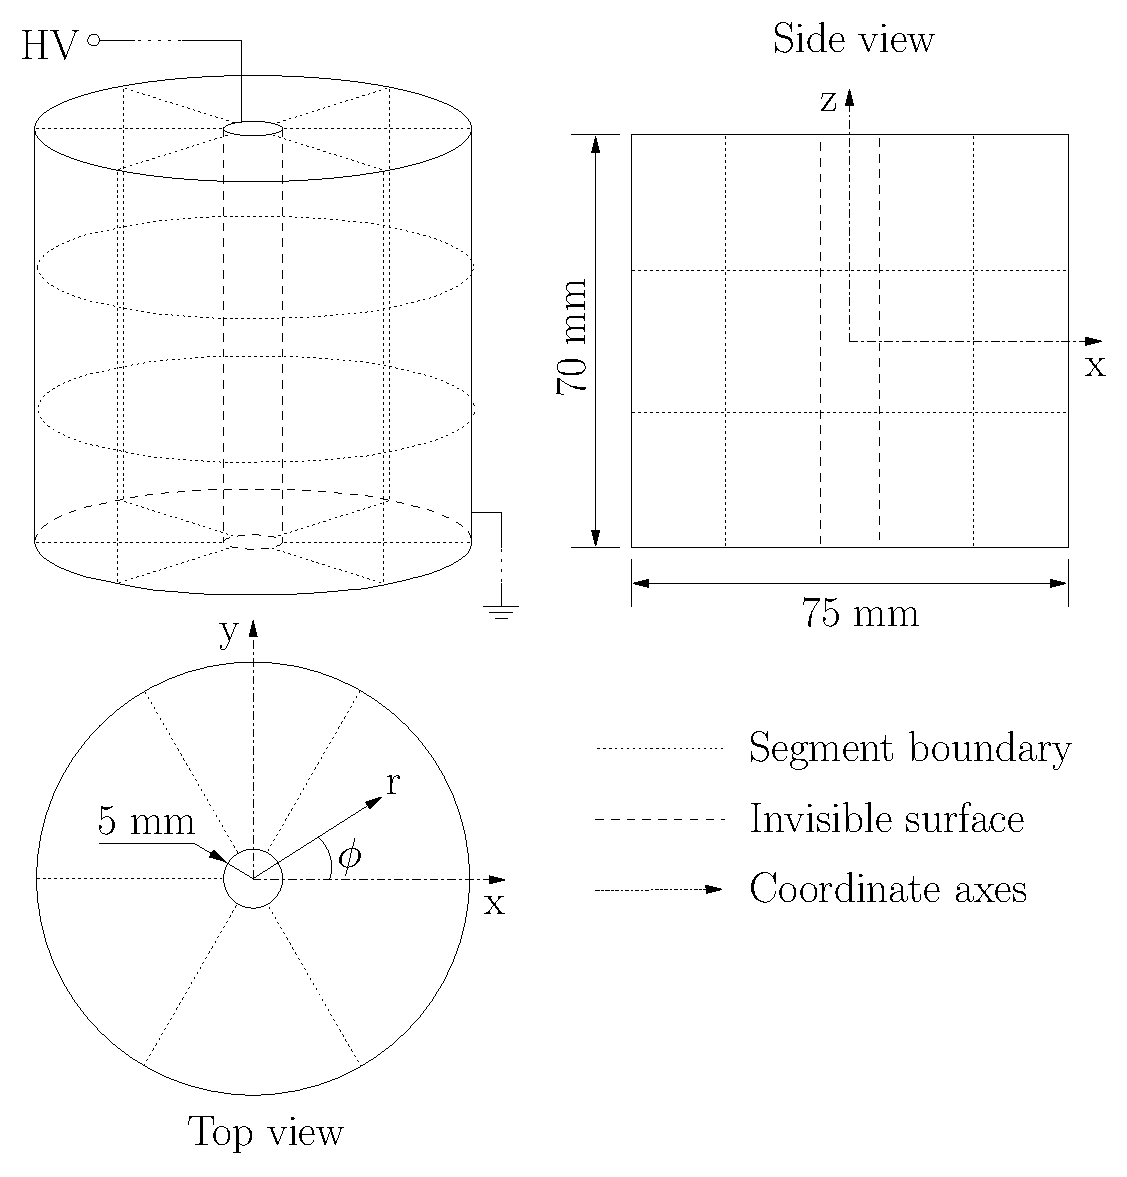
\includegraphics[width=0.85\linewidth]{model}
\caption{Detector model implemented in the simulation according to the
GERDA Phase~II prototype detector. The detector is equally separated
to six segments in $\phi$ and three segments in $z$.}
\label{f:model}
\end{figure}

The results of the comparison are planned to be presented in a series
of papers. This paper covers the detailed description of the
simulation methods and the verification of the simulation of pulses
induced by electrons drifting inside the germanium detector. The
verification of other aspects of the simulation, for example, the
drift of holes, will come with separated papers.

\section{Pulse shape simulation}
\label{s:pss}
\subsection{Procedure of the simulation}
\label{s:proc}
Particles ($\alpha, \beta, \gamma, n, p$, etc.) interacting inside
semiconductor detectors create electron-hole pairs, which act as
charge carriers. Due to the electric field inside the detector the
charge carriers drift and induce electric signals in the
electrodes. The electric signals are amplified, digitized and recorded
by the electronics and data acquisition systems connected to the
detector. The procedure to simulate this signal formation process in
germanium detectors hence can be naturally designed as follows:
\begin{enumerate} 
\item Simulate the interactions of particles with germanium to obtain
the positions and the energy deposits of the interactions (hits);
\item Group hits if they are closer to each other than the spatial
resolution of the detector. The position of the new hit is the
barycenter of the energies of the original hits. The energy of the new
hit, $E_{\mbox{hit}}$, is the sum of the energies of the original
hits. The number of electron-hole pairs created by the new hit is $n =
E_{\mbox{hit}} / E_{\mbox{pair}}$ with the pair energy
$E_{\mbox{pair}} = 2.95$~eV;
\item Calculate the electric field inside the detector according to
the geometry of the detector, the high voltage applied and the spatial
distribution of the impurity.
\item Calculate the trajectories of electrons and holes drifting from
the interaction point to the electrodes of the detector taking into
account the effect of the germanium crystal structure;
\item Calculate the time development of the charges, namely, the
pulses, induced in the electrodes by the drift of the charge carriers
based on Shockley-Ramo's Theorem \cite{Gat82,Rad88,He00}.
\item Add the effects from the electronics such as noise, bandwidth
limit, and shaping, etc. to the simulated pulses.
\end{enumerate} 
The first step is done using a Geant4 \cite{G403,G406} based
simulation package MaGe \cite{MaGe}, jointly developed by the GERDA
and Majorana collaborations. Steps 3-6 are covered in the following
sections.

\subsection{Electric field}
\label{s:field}
The electric field, $\vec{E}$, could in principle be calculated by
solving analytically Poisson's equation $\nabla \cdot \vec{E} =
\frac{\rho}{\epsilon}$, where $\rho$ is the space charge density
defined by the effective number of impurities and $\epsilon$ is the
dielectric constant. It is more practical to numerically calculate the
potential field $\varphi$ with certain boundary conditions. For
true-coaxial $n$-type detectors the potential is several kilo volt on
the inner surface, zero on the outer surface and float on the end
surfaces. The electric field is then obtained using $\vec{E} = -
\nabla \varphi$. It is convenient to use cylindrical coordinates, $r,
\phi, z$, in case of true-coaxial detectors:
\begin{equation} 
\frac{1}{r} \frac{\partial \varphi}{\partial r} + 
\frac{\partial^{2} \varphi}{\partial r^{2}} + 
\frac{1}{r^{2}} \frac{\partial^{2} \varphi}{\partial \phi^{2}} + 
\frac{\partial^{2} \varphi}{\partial z^{2}} = 
- \frac{\rho}{\epsilon_{0} \epsilon_{R}}, 
\label{e:pocyl} 
\end{equation} 
where $\varphi$ and $\rho$ are functions of $r, \phi, z$;
$\epsilon_{0}$ and $\epsilon_{R}$ are the dielectric constants in
vacuum and germanium, respectively.

Since the electric field does not change during the simulation, it is
calculated before the simulation and saved into a binary file. When
needed the file can be read in, and the electric field at any position
inside the detector can be calculated by interpolating from the
closest grid points.
 
The electric field distribution inside the germanium crystal is quite
sensitive to the impurity density. Figure~\ref{f:rho} shows the
strength of the electric field as a function of $r$ with the bias
voltage fixed at 3~kV. A change of the impurity density by one order
of magnitude changes the electric field dramatically. Even a factor
three difference, usually allowed between top and bottom for a
commercial detector, has a very significant effect.
 
\begin{figure}[htbp]
\centering
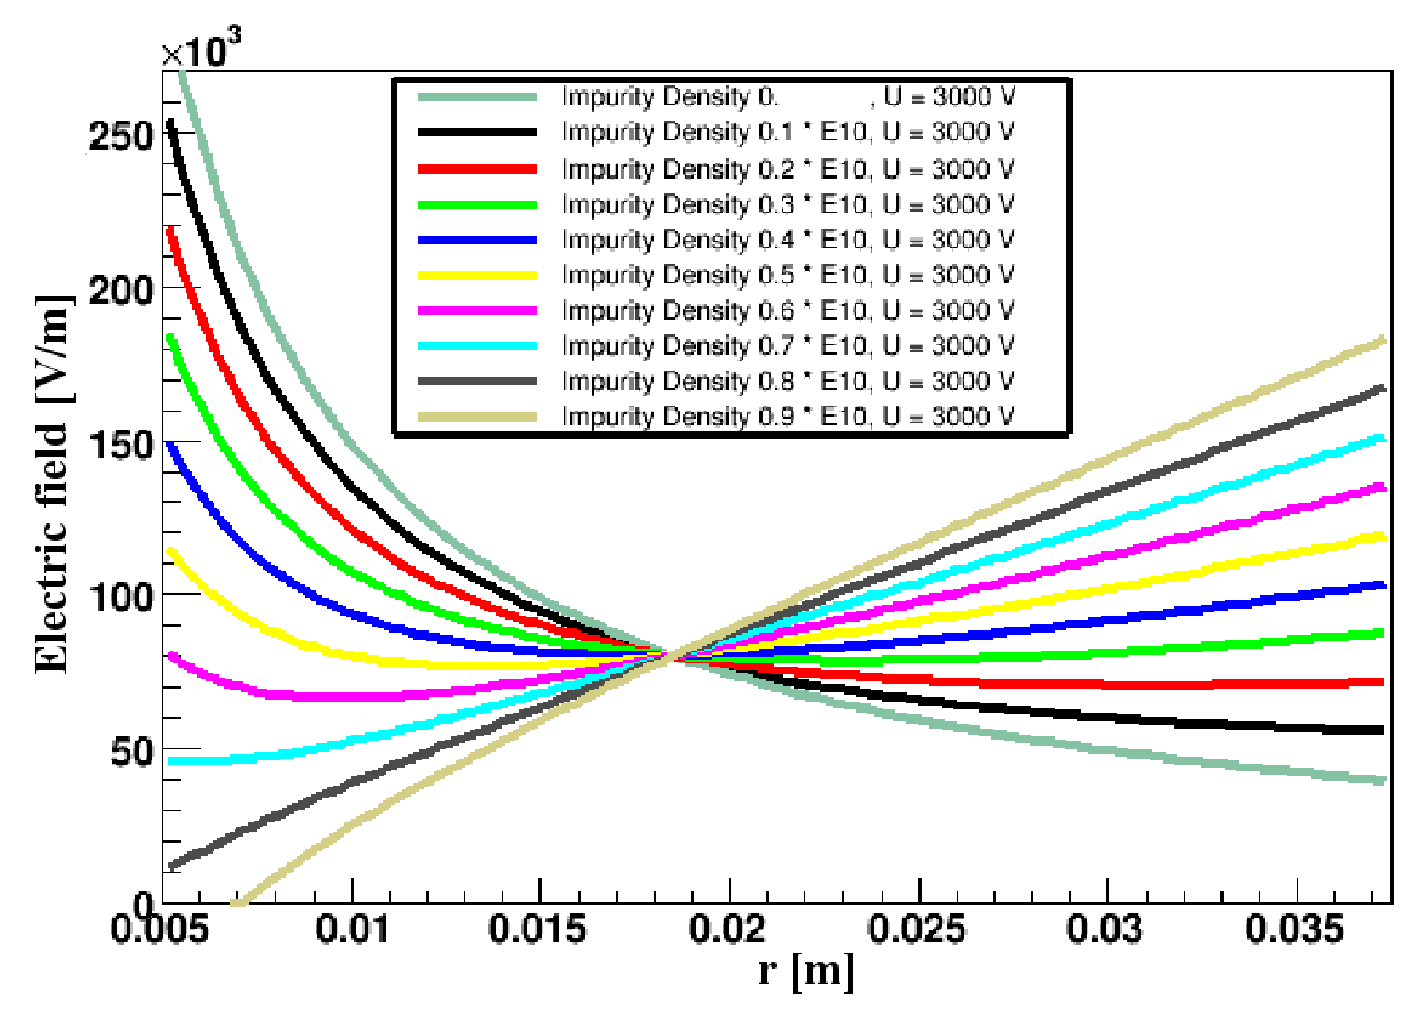
\includegraphics[width=\linewidth]{rho} 
\caption{Strength of the electric field as a function of the
cylindrical coordinate $r$ for impurity densities between 0 and $0.9
\times 10^{-10}$/cm$^{3}$.}
\label{f:rho} 
\end{figure}

The dielectric constant $\epsilon_{R}$ changes slightly with
temperature, strength of the electric field and frequency of the
signal. A detailed investigation is going on. For this application a
fixed value 16 was taken from page~357 of \cite{Kno99}. The effect of
diviation from this value can be absorbed into a redefinition of the
space charge density.

\subsection{Drift of charge carriers} 
\label{s:drift} 
\subsubsection{Mobility} 
\label{s:mobi} 
The relation between the drift velocity of the charge carriers,
$\vec{v}_{e}(\vec{r})$ for electrons and $\vec{v}_{h}(\vec{r})$ for
holes, and the electric field, $\vec{E}(\vec{r})$, can be simply
expressed as:
\begin{equation} 
\label{e:dv}
\vec{v}_{e/h} (\vec{r})= \mu_{e/h} \vec{E}(\vec{r}),
\end{equation}
where $\mu_{e/h}$ is called the \emph{mobility} and $\vec{r}$
indicates the position. The mobility changes with the temperature of
the germanium crystal. If the temperature\footnote{If the velocities
of a group of particles follow a Maxwell-Boltzmann distribution, their
temperature is defined as the temperature of that distribution.} of
the crystal lattice is the same as that of the charge carriers, the
crystal structure has no influence on the drift. The drift velocity is
proportional to the electric field so the mobility in this case is
just a number. Since germanium detectors are normally operated at
liquid nitrogen temperature ($\sim78$~K), the crystal lattice has
lower temperature than the charge carriers and affects on their
drift. The drift velocity hence is not always parallel to the electric
field and the mobility in this case is a complex tensor.

Germanium has the same crystalline structure as silicon and diamond,
namely, a face-centered cubic (FCC) structure: each atom is at the
center of a regular tetrahedron and is surrounded by four atoms as
shown in Fig.~\ref{f:xtal}. Also shown is the definition of crystal
axes in terms of the Miller index.
\begin{figure}[htpb]
\centering
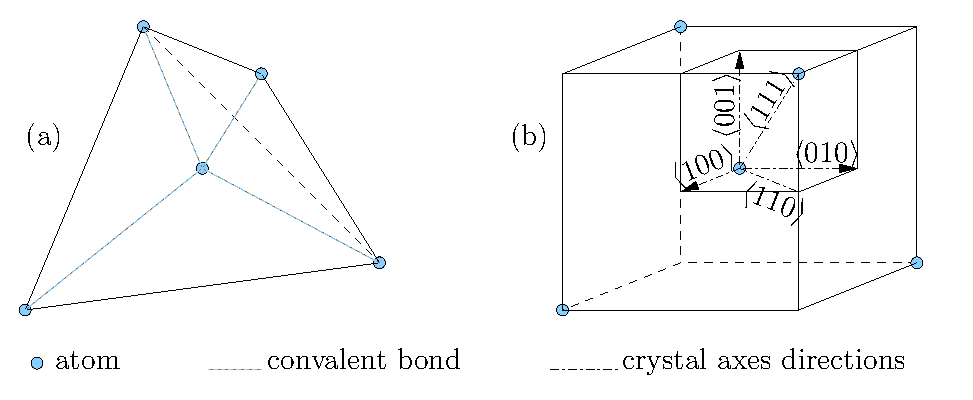
\includegraphics[width=\linewidth]{xtalStruc}   
\caption{Structure of germanium crystals: (a) basic configuration and
(b) definition of crystal axes.}
\label{f:xtal} 
\end{figure} 

Germanium detectors with cylindrical shapes are produced with their
geometrical center axis, $z$, aligned to the crystal axis $\langle 001
\rangle$, as shown in Fig.~\ref{f:coo}. The transformation between
$xyz$ and the coordinate system defined by the crystal axes $\langle
100 \rangle$, $\langle 010 \rangle$ and $\langle 001 \rangle$ only
depends on the angle between the $\langle 110 \rangle$ and the y-axis,
$\phi_{110}$.
\begin{figure}[htpb]\sidecaption
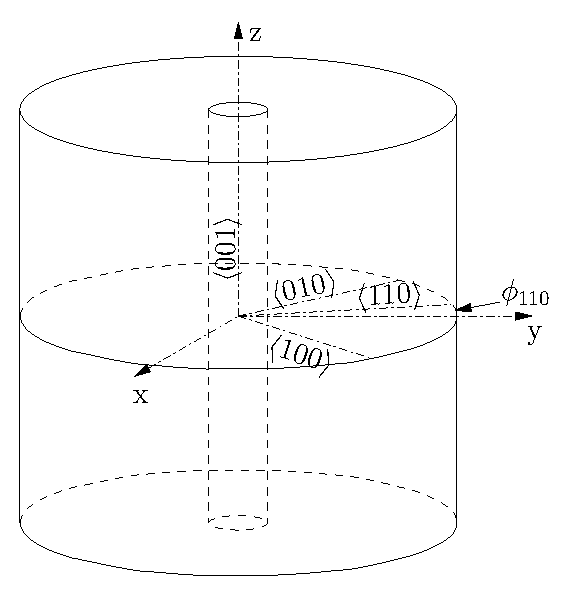
\includegraphics[width=0.55\linewidth]{coordins}
\caption{Relation between the coordinates $xyz$ and the crystal
axes $\langle 100 \rangle$, $\langle 010 \rangle$ and $\langle 001
\rangle$.}
\label{f:coo} 
\end{figure} 
 
If the electric field lines are parallel to any of the principal
crystallographic axes, charge carriers will always drift along the
electric field despite of the lattice temperature because of the
symmetric structure of the germanium crystal. Measurements of the
drift velocities along the axes $\langle 100 \rangle$ and $\langle 111
\rangle$ with electric fields parallel to them were performed
\cite{miha,reg,bart} and the data can be fitted well by the following
parametrization \cite{Kno99} with electric field strengths below
300~V/mm \cite{miha}:
\begin{equation} 
\label{e:para} 
v = \frac{\mu_{0}E}{[1+(\frac{E}{\mathcal{E}_{0}})^{\beta}]^{1/\beta}}, 
\end{equation} 
where $v$ and $E$ are the magnitudes of the drift velocity and the
electric field, respectively, $\mu_{0},\mathcal{E}_{0}$ and $\beta$
are parameters to be determined by fitting. The parameter $\mu_{0}$
represents the linear relation between $v$ and $E$ at high lattice
temperatures and low electric fields, while the parameters
$\mathcal{E}_{0}$ and $\beta$ model the deviation from this linear
relation at low lattice temperature and high electric fields. The
values of the parameters from the fit to the experimental data are
listed in Table~\ref{t:pars}. Equation~\ref{e:para} with the input
parameters listed in Table~\ref{t:pars} is visualized in
Fig.~\ref{f:vvse}.

The set of parameters given in \cite{bart} was used in the simulation
presented here. Because it was verified with data taken with two AGATA
\cite{agata} prototype detectors, and proven to be reliable,
especially for the drift of electrons \cite{bart2}.
 
\begin{table}[htpb]
\centering
\caption{Parameters for the experimental drift velocities in the
$\langle111\rangle$ and $\langle 100 \rangle$ directions
(taken from Ref.~\cite{bart}).}
\label{t:pars}
\begin{tabular}{cccccc}
\hline\noalign{\smallskip}
Ref. & Carrier & Axis &
$\mu_{0} \left[\frac{\mbox{cm}^{2}}{\mbox{V}\cdot\mbox{s}}\right]$ &
$\mathcal{E}_{0}\left[\frac{\mbox{V}}{\mbox{mm}}\right]$ & $\beta$\\
\noalign{\smallskip}\hline\noalign{\smallskip}

\multirow{2}{*}{\cite{miha}}&\multirow{2}{*}{$e$} &
$\langle111\rangle$ & 42420 & 25.1 & 0.87 \\
& & $\langle100\rangle$ & 40180 & 49.3 & 0.72 \\
\noalign{\smallskip}\hline\noalign{\smallskip}

\multirow{2}{*}{\cite{reg}}&\multirow{2}{*}{$h$} &
$\langle111\rangle$ & 107270 & 10.0 & 0.580 \\
& & $\langle100\rangle$ & 66333 & 18.1 & 0.744 \\
\noalign{\smallskip}\hline\noalign{\smallskip}

\multirow{4}{*}{\cite{bart}}&\multirow{2}{*}{$e$} &
$\langle111\rangle$ & 38536 & 53.8 & 0.641 \\
& & $\langle100\rangle$ & 38609 & 51.1 & 0.805 \\
\noalign{\smallskip}\cline{2-6}\noalign{\smallskip}

&\multirow{2}{*}{$h$} & $\langle111\rangle$ & 61215 & 18.2 & 0.662 \\ 
& & $\langle100\rangle$ & 61824 & 18.5 & 0.942 \\
\noalign{\smallskip}\hline\noalign{\smallskip}
\end{tabular} 
\end{table}
 
\begin{figure*}[tb]
\centering
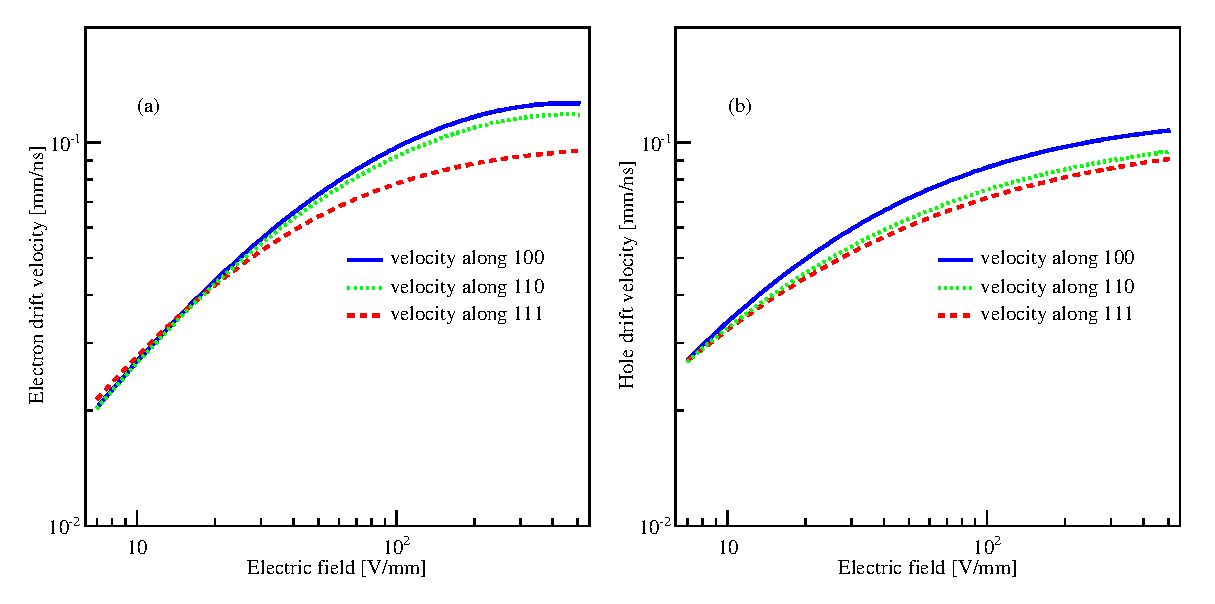
\includegraphics[width=0.8\linewidth]{VvsElucian} 
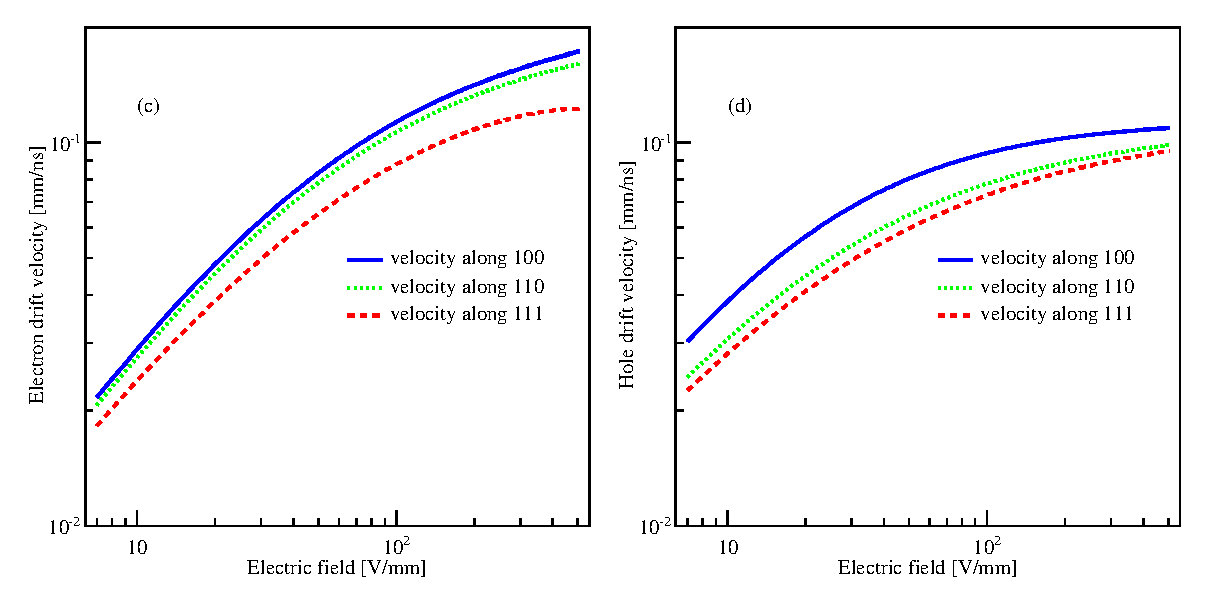
\includegraphics[width=0.8\linewidth]{VvsEbart} 
\caption{Drift velocities of electrons (a, c) and holes (b, d) along
the principal crystal axes as functions of the electric
field. Velocities along the axes $\langle 100 \rangle$ and $\langle
111 \rangle$ are calculated according to Eq.~\ref{e:para}: (a) and
(b), the input parameters provided in \cite{miha} and \cite{reg} are
used; (c) and (d), the input parameters provided in \cite{bart} are
used. The velocities along the $\langle 110 \rangle$ axis are
predicted according to Sect.~\ref{s:elec} and~\ref{s:hole}.}
\label{f:vvse} 
\end{figure*} 

\subsubsection{Drift velocities}
\label{s:vel}
The drift velocity in an arbitrary direction can be derived from the
velocities along the $\langle 100 \rangle$ and $\langle 111 \rangle$
axes given by Eq.~\ref{e:para}.

The model used to calculate the electron drift velocity in any
direction is taken from \cite{miha} and references therein. The basic
idea is, that the conduction band in a germanium crystal reaches its
minimal potential in regions around the four equivalent $\langle 111
\rangle$ axes; free electrons can easily populate in these regions and
accelerated by the electric field; the probability density of free
electrons in other regions is very small and can be ignored. Detailed
calculation is described in Appendix~\ref{s:elec}. The electron drift
velocities along the $\langle 110 \rangle$ axis are calculated as
examples, and shown as the dotted lines in Fig.~\ref{f:vvse}a and c.

The model used to calculate the hole drift velocity in any direction
is taken from \cite{bart} and the references therein. The basic idea
is, that only the \emph{heavy hole valence band} \cite{heavy} is
responsible for the anisotropy of the mobility, all other effects are
neglected, and that the mean wave vector $\vec{k}_{0}$ of heavy holes
is aligned with the electric field $\vec{E}$. Detailed explanation can
be found in Appendix~\ref{s:hole}. The hole drift velocities along the
$\langle 110 \rangle$ axis are calculated as examples, and shown as
the dotted lines in Fig.~\ref{f:vvse}b and d.

\subsubsection{Drift trajectories} 
\label{s:trj} 
The development of the drift are calculated iteratively. The
displacement vector $\Delta \vec{r}$ by which charge carriers drift
within a short time interval $\Delta t$ can be calculated once the
drift velocity vector $\vec{v}_{i}$ in the prior position
$\vec{r}_{i}$ is calculated using the method described in the previous
two sections.  The new position $\vec{r}_{i+1}$ is then
\begin{equation} 
\label{e:pos} 
\vec{r}_{i+1} = \vec{r}_{i} + \Delta \vec{r} \ \ 
(i=0,1,...), \mbox{ with } 
\Delta \vec{r} = \vec{v}_{i} \Delta t. 
\end{equation} 
The iteration continues until the charge carriers reach the boundary
of the crystal, denoted as $\vec{r}_{b}$. The series of position
vectors, $(\vec{r}_{0}, \vec{r}_{1}, ..., \vec{r}_{i}, ...,
\vec{r}_{b})$, represents the drift trajectory.
 
Two different numerical methods are implemented to calculate the
trajectory, the Euler method and the 4$^{th}$ Runge-Kutta method. The
former is less computer time intensive, but is also less precise.
However, for time intervals $\Delta t \lesssim 1$~ns, the output of
the two methods does not differ significantly. The results presented
here are obtained with the Runge-Kutta method.
 
Figure~\ref{f:trjs} shows the drift trajectories projected on an x-y
cross section of the detector. The crystal axis $\langle 110 \rangle$
is set to be parallel to the y-axis. The left plot shows the inward
drift of electrons starting at the outer surface of the detector. The
starting points are distributed equidistantly on the outer circle.
The right plot shows the outward drift of holes starting at the inner
surface. The starting points are distributed equidistantly on the
inner circle. The bias voltage is set to 3000~V. The time interval is
1~ns. The time window for the development of the drift is 400~ns. All
electrons reach the inner surface within this time window, but not all
holes reach the outer surface, demonstrating the longitudinal
anisotropy of the drift. This is because electrons drift faster than
holes, and holes drift slowest along the $\langle 110 \rangle$
direction, as also shown in Fig.~\ref{f:vvse}. The trajectories along
the crystal axes are straight because of the symmetry of the crystal
structure. However, they are clearly bent along other directions,
demonstrating the transverse anisotropy of the drift.
\begin{figure*}[tb]
\centering
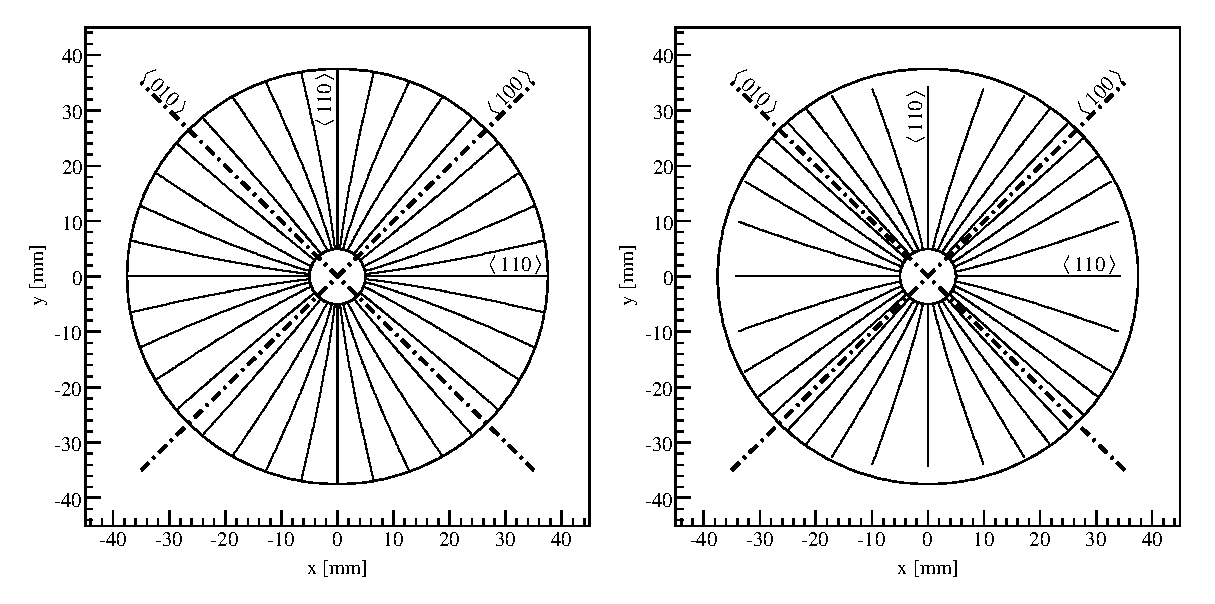
\includegraphics[width=0.8\linewidth]{trjs} 
\caption{Drift trajectories projected on the x-y cross sections of the
detector: Left, electrons drift inward; Right, holes drift outward.}
\label{f:trjs} 
\end{figure*} 
 
\subsection{Weighting potentials and fields}
\label{s:wei}
Electric signals are induced in the electrodes of a detector by the
cumulative influence of electrons and holes moving toward the
electrodes. Shockley-Ramo's Theorem \cite{Gat82,Rad88,He00} can be
used to calculate the time development of the induced charge $Q(t)$ or
current $I(t)$ in each electrode:
\begin{equation} 
\label{e:ramoq}
Q(t) = -Q_{0} \times [\varphi_{w}(\vec{r}_{h}(t)) -
\varphi_{w}(\vec{r}_{e}(t))],
\end{equation}
\begin{equation} 
\label{e:ramoi}
I(t) = Q_{0} \times [\vec{E}_{w}(\vec{r}_{h}(t)) \cdot 
\vec{v}_{h}(t) - \vec{E}_{w}(\vec{r}_{e}(t)) \cdot 
\vec{v}_{e}(t)],
\end{equation}
where $Q_{0}$ is the electric charge carried by electrons or holes,
$\vec{r}_{e/h}(t)$ and $\vec{v}_{e/h}(t)$ are the position and
velocity vectors of electrons/holes as a function of time, and
$\varphi_{w}$ and $\vec{E}_{w}$ are the \emph{weighting potentials}
and \emph{weighting fields}.

The weighting potentials and fields can be calculated by solving
Poisson's equations, $\nabla^{2} \varphi = 0$ and $\nabla \cdot
\vec{E} = 0$, respectively, with the boundary conditions that the
potential on the electrode of interest equals to 1 and the potentials
on all other electrodes equal to zero. Just like the electric fields,
they are calculated before the simulation in a grid, and saved to a
binary file for later interpolation.

Figure~\ref{f:psh} shows the weighting potential of a segment with the
indication of a photon event. Figure~\ref{f:pss} shows the raw charge
and current pulses induced by the resulting hit in this particular
segment, its neighboring segments and the core of the detector. The
pulses induced in the neighboring segments are called \emph{mirror
pulses}. The amplitude of the mirror pulse induced in one neighboring
segment is larger than in the other, because the trajectory of the hit
is closer to this segment.
\begin{figure*}[tb] 
\centering 
\subfloat[]{\label{f:psh} 
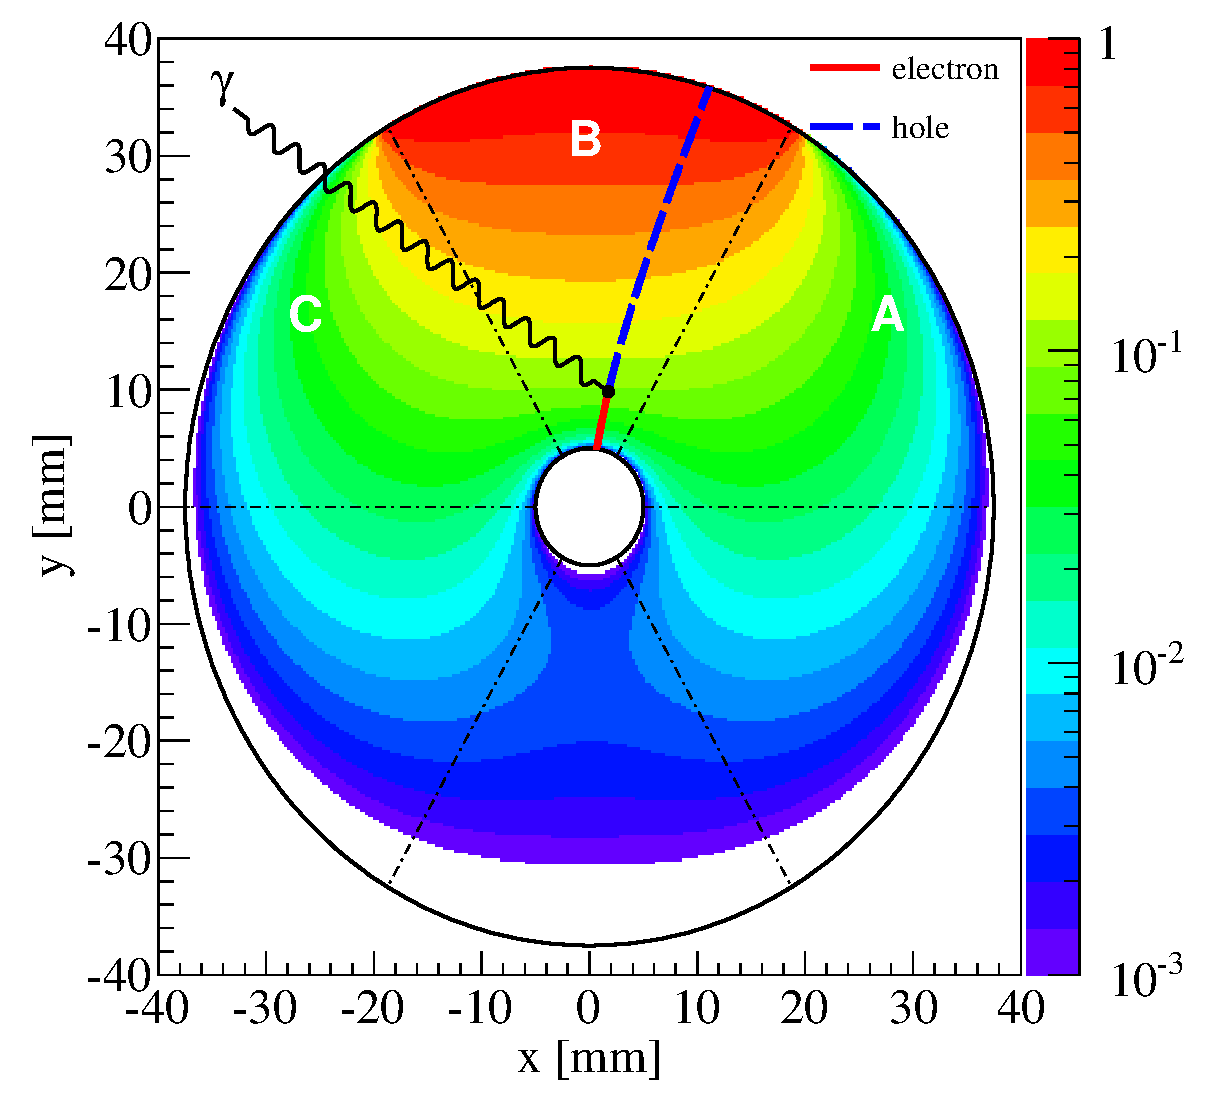
\includegraphics[height=0.235\textheight]{WP}}% 
\subfloat[]{\label{f:pss} 
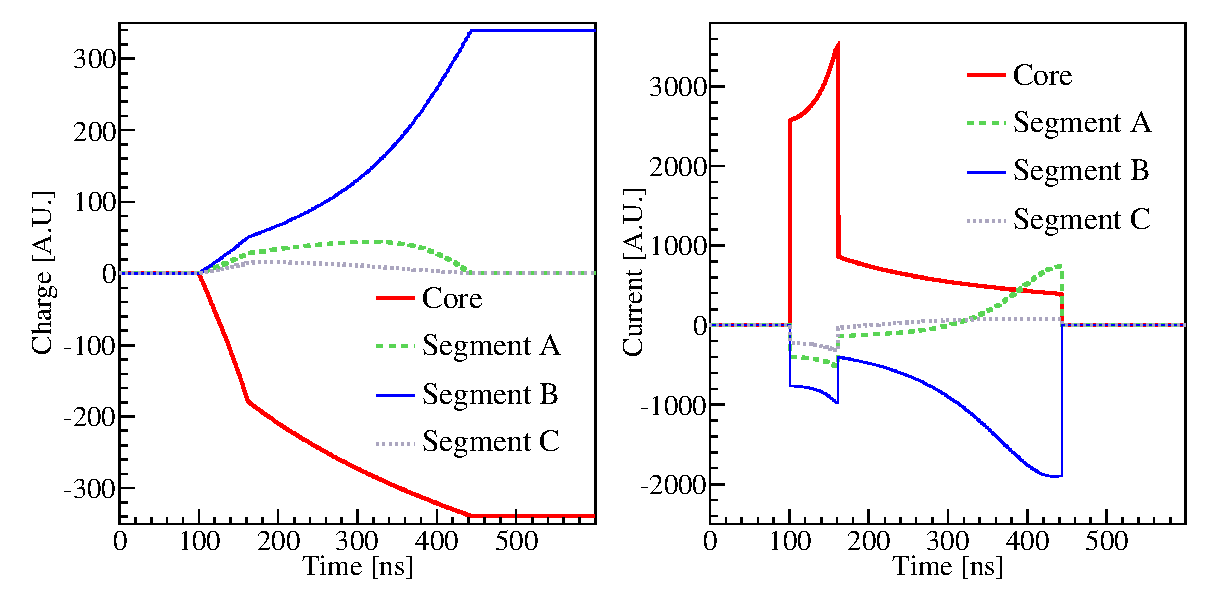
\includegraphics[height=0.235\textheight]{CIPS}}% 
\caption{(a) weighting potential of segment B together with an
indication of a $\gamma$ interaction. (b) Simulated charge and current
pulses induced in segments A, B and C.}
\label{f:ps} 
\end{figure*} 

\subsection{Effects of electronics} 
\label{s:dbn}
The pulses recorded by the DAQ system are quite different from the raw
pulses. Not only their amplitudes but also their shapes are changed by
the electronics. The signal falls exponentially to its baseline with a
time constant $\tau$. The limit on the bandwidth of the signal
transmission through the electronics cuts off the signal components
with frequencies higher than the limit. Sharp edges in a pulse are
hence smeared. Electronic noise may destroy any detailed structure of
a pulse. All these effects need to be simulated.
 
Figure~\ref{f:elec} shows a modified pulse after folding in the decay
of the signal, the limited bandwidth and the noise. The decay time was
$5 \mu$s, the cut-off in bandwidth was 10~MHz and the noise level was
5\% of the pulse amplitude. These values are worse than those were
observed in the test stand for the first GERDA Phase~II prototype
detector~\cite{si}. They were chosen to clearly demonstrate the
effects.
\begin{figure}[htpb]
\centering
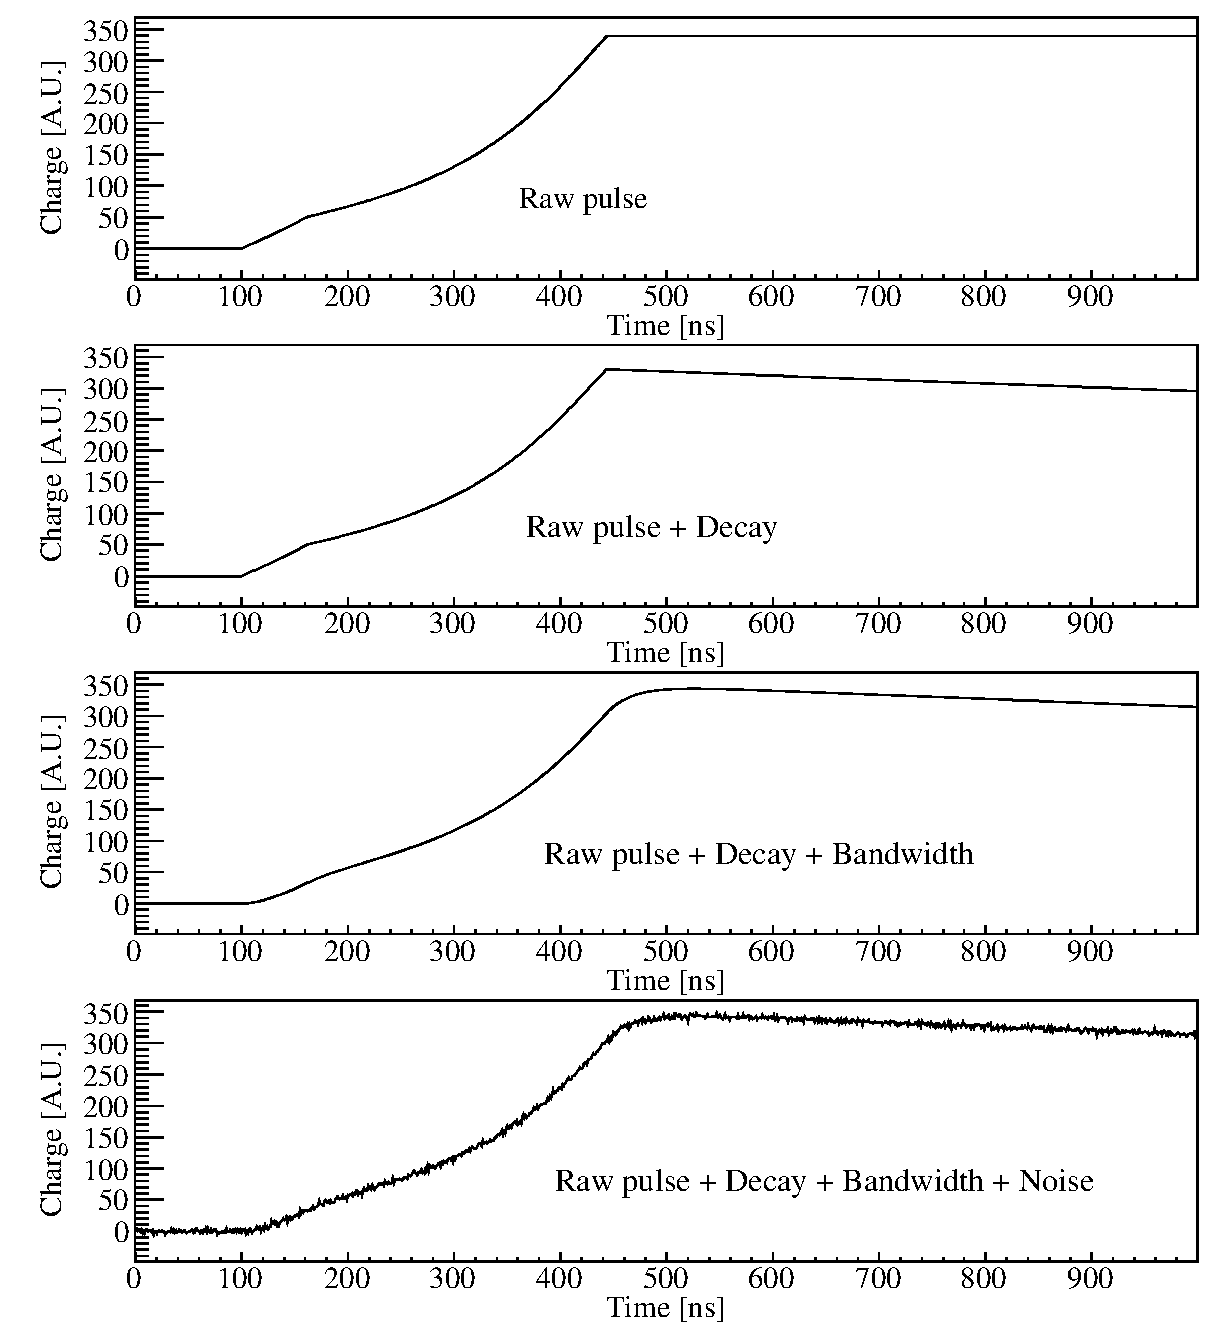
\includegraphics[width=\linewidth]{PSDBN} 
\caption{Modified pulses after folding in the decay of the signal, the
limited bandwidth and the noise.}
\label{f:elec} 
\end{figure}

\section{Validation of the simulation}
\label{s:psv}
The physics models \cite{miha,bart} for the drift of charge carriers
and their measured input parameters \cite{miha,reg,bart} alone are not
enough to provide a realistic pulse shape simulation. While some input
parameters are generic to germanium, others, like the impurity density
and the detailed properties of the surface layers, are different for
each detector. Normally the information of these properties provided
by the detector manufacturer is not accurate enough for a precise
pulse shape simulation. The comparison of the simulation with data
taken with an individual detector would improve the knowledge of these
important properties of the detector. The simulation can then be tuned
accordingly for the individual detector or for a series of similar
detectors.

In most of the cases, pulses are induced by both electrons and holes
drifting towards the electrodes. A common way to separate the effects
of electrons from those of holes is to scan the surfaces of the
detector with a low energy $\gamma$ source. Because low energy photons
in average do not penetrate deeply into germanium and most likely
deposit energy locally through the photoelectric effect, they create
electron-hole pairs predominantly near the surface of the
detector. One type of charge carrier reaches the near surface almost
immediately while the other drifts through the whole bulk of the
detector to reach the far surface. Therefore, the pulse shapes are
mainly determined by one type of charge carrier.

Pulses mainly induced by electrons can be collected by scanning the
outer surface of an $n$-type detector. This was done with the first
GERDA Phase~II prototype detector. \cite{si} The pulse shape
simulation was verified using these data. The results are presented in
this section.

\subsection{Measurement}
\label{s:char}
The measurement was done as shown in Fig.~\ref{f:siscan}. The surfaces
of segments 13, 14 and 15\footnote{labeled according to the channel
number provided by the detector manufacturer} in the middle layer of
the detector were scanned in azimuth angle, $\phi$\footnote{defined by
the protractor used in the measurement} using a 75~kBq $^{152}$Eu
source inside a copper collimator with a length of 52~mm and a
pin-hole diameter of 11~mm. The distance between the collimator and
the center of the detector was $\approx 85$~mm. The spot size on the
detector surface was estimated to be $\approx 150$~mm$^{2}$. The
center of the collimator was pointed at $z = 0$. The step size of the
scan was 5$^{\circ}$ in segment 14 and 10$^{\circ}$ in segment 13 and
15. The uncertainty in $\phi$ is $\approx \Delta \phi=2.5^{\circ}$. In
total 25~measurements were performed to cover 180$^{\circ}$ in
azimuth. The pulses of the core and all segments were recorded.

\begin{figure}[htbp]
\centering
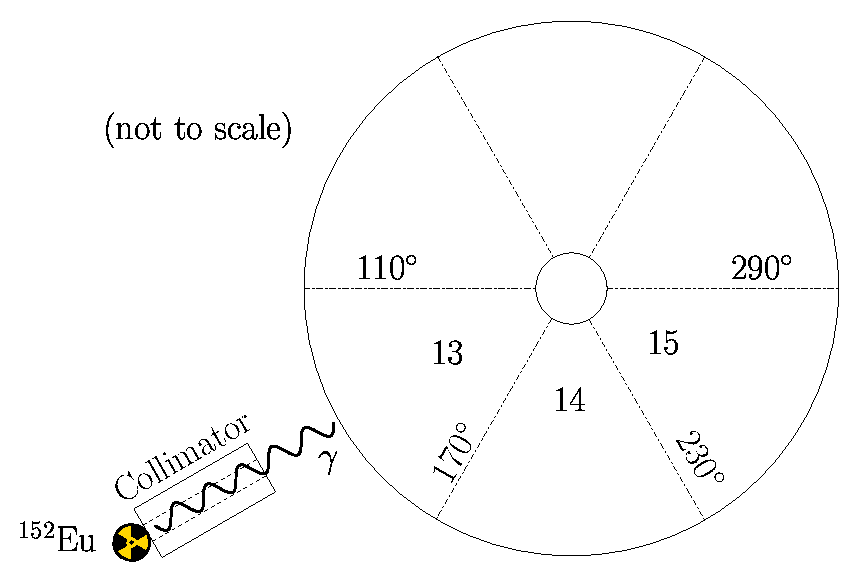
\includegraphics[width=0.8\linewidth]{siscan}
\caption{Scan on the surface of a GERDA Phase II prototype detector.}
\label{f:siscan}
\end{figure}

The 122~keV $\gamma$ line of the $^{152}$Eu source used in the scan
provided the events to study the drift of electrons. 

\subsection{Rise time comparison}
\label{s:lon}
To analyze the pulse shapes quantitatively the 10\%-30\% and 10\%-90\%
risetimes of the core pulses were calculated. Figure~\ref{f:rt10}
shows the average risetimes as a function of the azimuth angle
$\phi$. The segment boundaries are also indicated.  Clear oscillation
patterns can be seen in both cases. This confirms the longitudinal
anisotropy of the drift velocity of electrons depending on the
angle~$\phi$. The electrons need different times to drift nearly the
same distance.\footnote{Strictly speaking, because of the bend of the
drift trajectories the distances covered by electrons in different
$\phi$ angles are sightly different from each other.  However, this is
a second-order effect. The difference of the risetimes is mainly
caused by the different drift velocity along $r$ at different angles
$\phi$.} Fits with a sine function give periods of about 90$^{\circ}$
for the longitudinal anisotropy. This supports the model applied.

\begin{figure}[htpb]
\centering
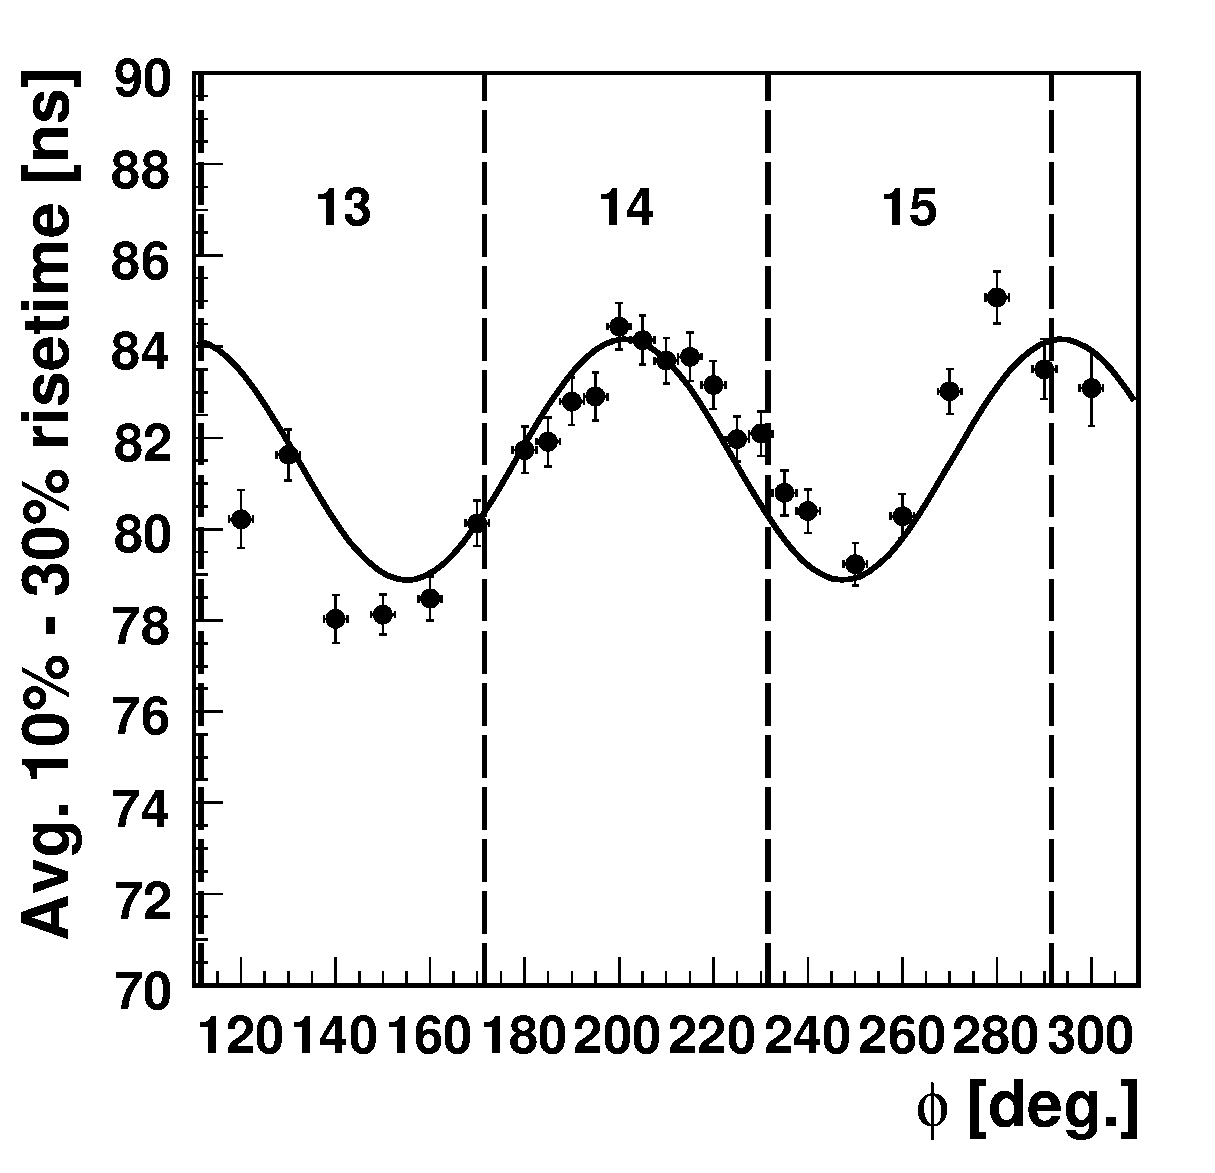
\includegraphics[width=0.7\linewidth]{phi_risetime1030}
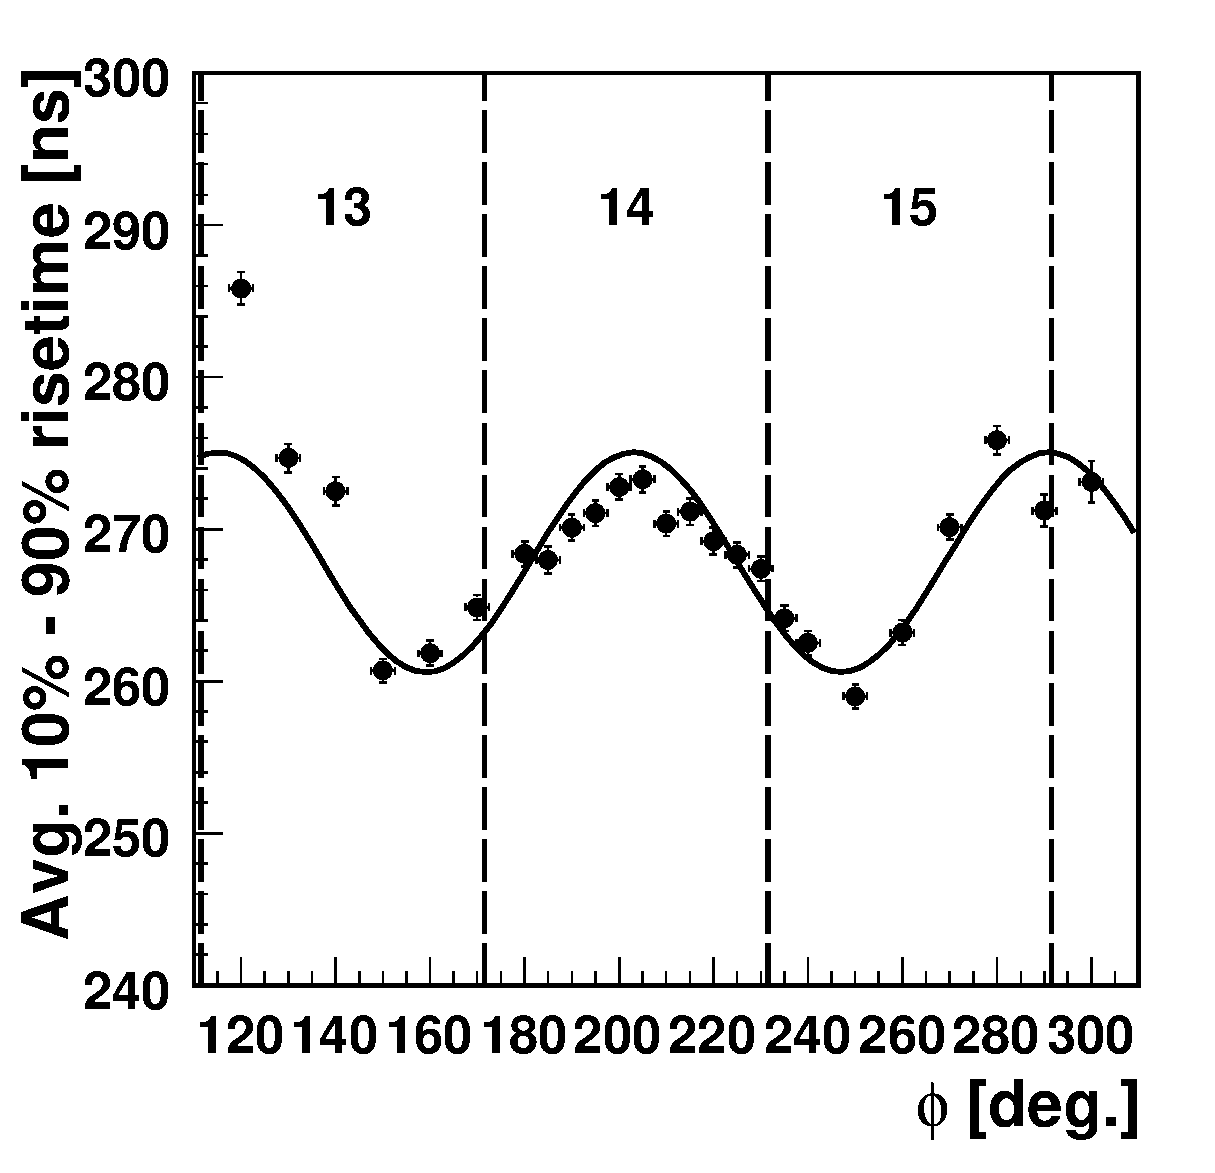
\includegraphics[width=0.7\linewidth]{phi_risetime1090}
\caption{Average 10\%-30\% (left) and 10\%-90\% (right) risetimes of
the core pulses as a function of the azimuth angle $\phi$ (taken from
\cite{si}). The dashed lines indicate the segment boundaries.}
\label{f:rt10}
\end{figure}

Pulses induced in the core electrode by the drift of electrons
starting at the outer surface of Siegfried I were simulated. The
geometry and the experimental setup implemented in the simulation are
shown in Fig.~\ref{f:model} and \ref{f:siscan}. The operational
voltage of Siegfried~I is 3~kV. The impurity density was implemented
in the simulation according to the values given by the detector
manufacturer.

According to the model, electrons drift slowest along the $\langle 110
\rangle$ axes and risetimes reach their maxima. Thus,
Figure~\ref{f:rt10} indicates that one of the $\langle 110 \rangle$
axes is nearly aligned with the right boundary of segment 15 at
$\approx$\,290$^\circ$. This was implemented in the simulation. A
decay time of 50~$\mu$s and a cut-off bandwidth of 37.5~MHz were
implemented according to the specification of the electronics
system. Electronic noise was not added to the pulse simulation to
simplify direct comparisons with individual pulses. Several
parameters, the \emph{Amplitude}, the \emph{Time offset} and the
\emph{Time scaling factor} of the pulse, were introduced to fit the
shape of a simulated to a measured pulse. The time offset shifts the
pulse while the time scaling factor stretches or squeezes the pulse in
time.

Figure~\ref{f:s2d} shows a randomly selected core pulse and the result
of a fit with the simulated pulse along the $\langle 110 \rangle$
axis. The fit yields a time scaling factor of 0.81, indicating that
the simulated pulse overestimates the pulse-length by $\approx
20\%$. Nevertheless the $\chi^{2}$/NDF is excellent. In general a
factor between 1 and 0.94 is expected as the simulation reflects the
maximal risetime.
\begin{figure}[htbp]
\centering
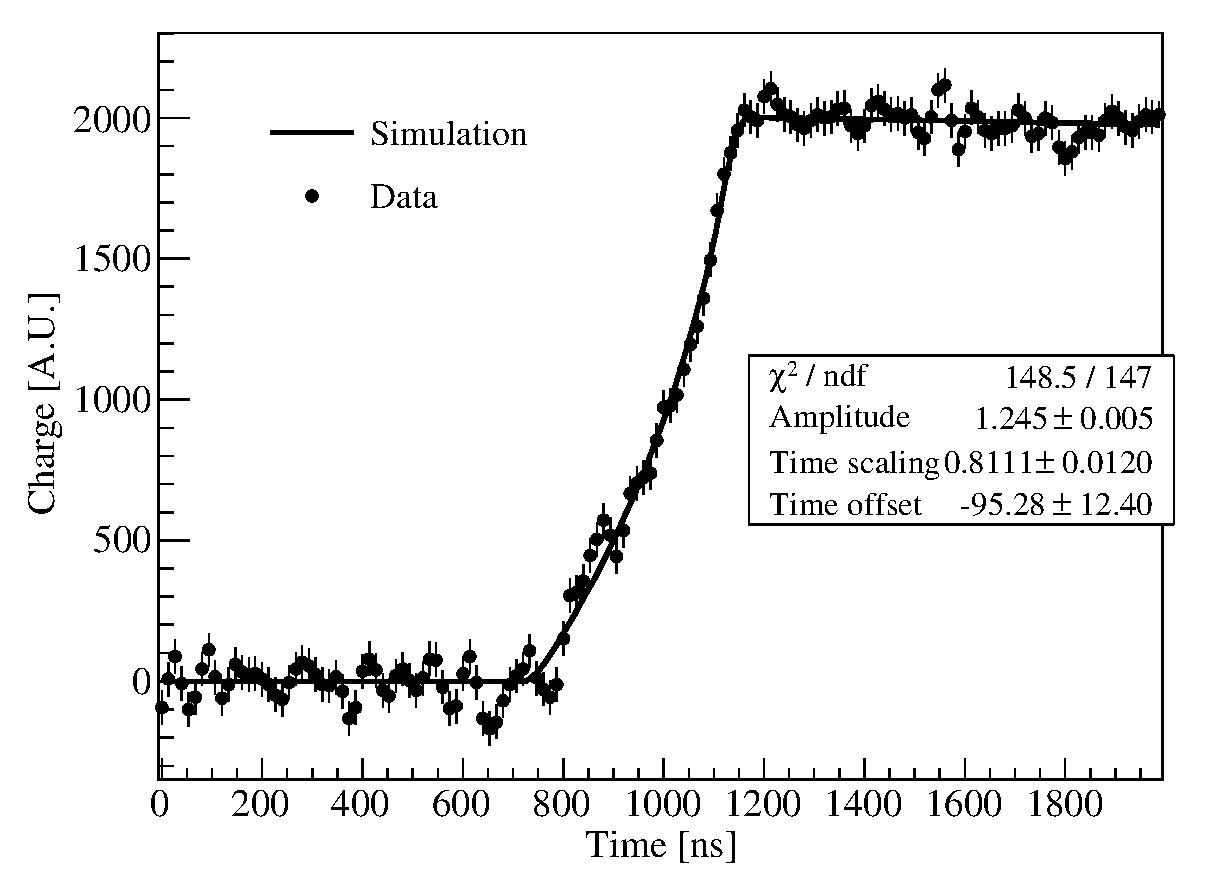
\includegraphics[width=\linewidth]{PSs2d}
\caption{Fit of a simulated to a measured pulse. The dots represent
the data and their error bars indicate the noise level.}
\label{f:s2d}
\end{figure}

A subset of pulses with fits were selected requiring
\begin{itemize}
\item $\chi^{2} < 200$ to eliminate very noisy events,
\item The pulse amplitude in simulation must be equal to that in data
within the resolution to eliminate events mis-recorded by the DAQ,
\item Time offset $> -300$~ns as very early pulses were not treated
correctly by the DAQ.
\end{itemize}

\begin{figure}[htbp]
\centering
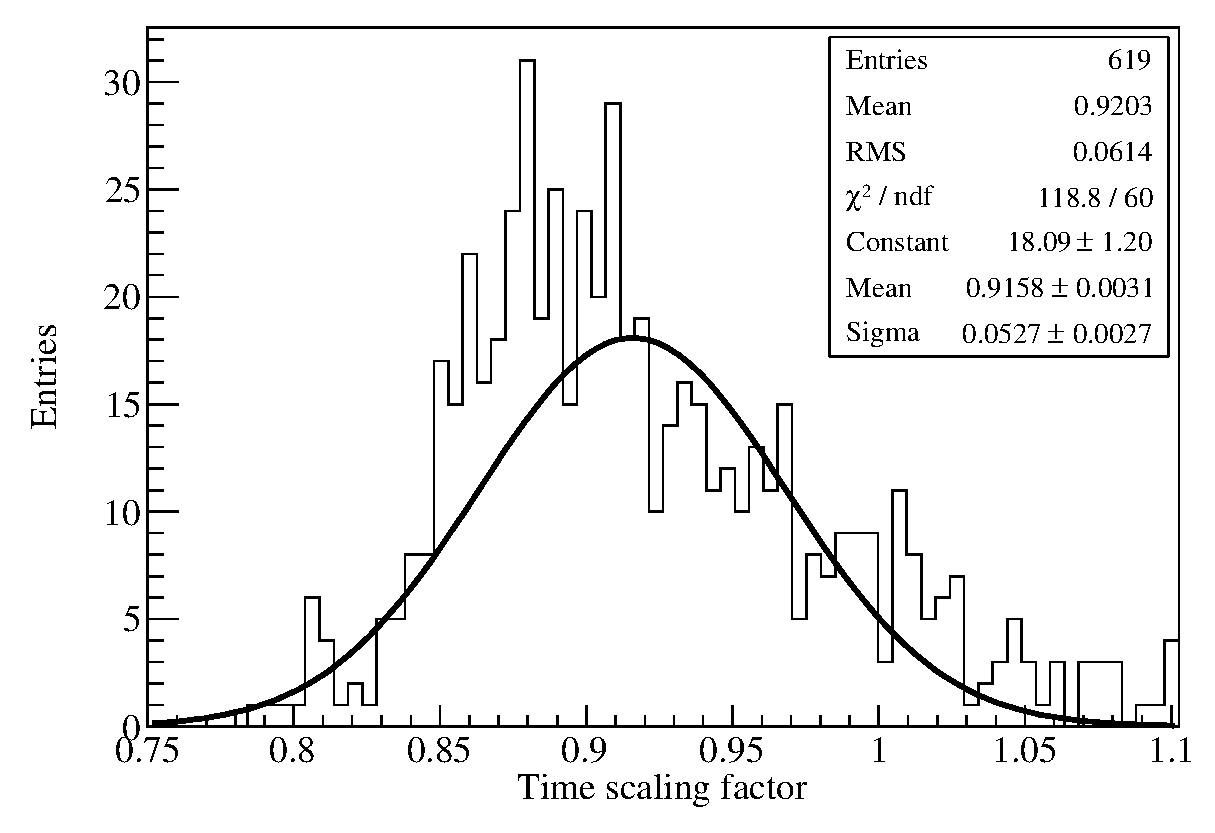
\includegraphics[width=0.9\linewidth]{tscale280}
\caption{Time scaling factors from the fits of the simulated to
measured pulses taken at $\phi=280^{\circ}$.}
\label{f:ts280}
\end{figure}

The distributions of the time scaling factors for each scan position
were fitted with a Gaussian function. Fig.~\ref{f:ts280} shows the
distribution for $\phi = 280^{\circ}$. The scaling factor at
$280^{\circ}$ should be close to one, if the model would represent the
detector perfectly. It is about 7\% lower. However, since the events
in data do not start exactly at the outer surface, slightly shorter
risetimes are expected in data compared to the simulation.

The mean scaling factors obtained from the fits versus azimuth are
displayed in Fig.~\ref{f:tsc}. The points were fitted with a sine wave
plus a 1$^{st}$-order polynomial. The period of the sine wave was
fixed to $90^{\circ}$. The shifted polynomial is shown as a baseline
in Fig.~\ref{f:tsc}. The data is reasonably well described by the
fit. However, the different values obtained for different instances of
the $\langle 110 \rangle$ configuration indicate that the actual
detector is more complex than assumed. One possible interpretation is
that the impurity density given by the manufacturer is an average
density and in reality varies with the azimuthal angle $\phi$.

\begin{figure}[htpb]
\centering
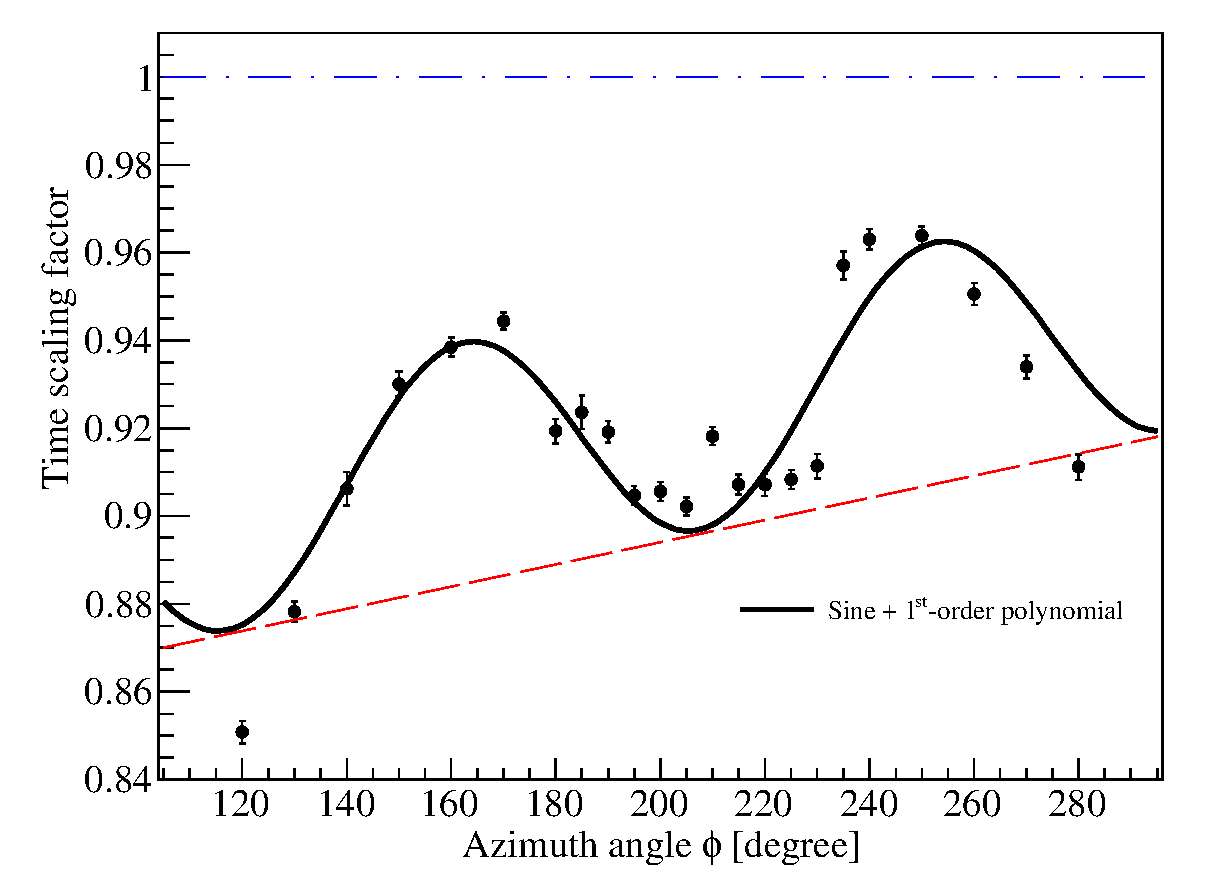
\includegraphics[width=\linewidth]{tsc}
\caption{Mean time scaling factor (black dots) of a simulated $\langle
110 \rangle$ pulse versus azimuth. The solid line represents a fit
with a sine wave plus a 1$^{st}$-order polynomial. The dashed line
shows the shifted polynomial as a baseline.}
\label{f:tsc}
\end{figure}

The oscillation pattern expected and seen in Fig.~\ref{f:tsc} should
disappear when the pulses are simulated for the individual angular
configuration of the the scan points. This was done and the result is
depicted in fig.~\ref{f:tsl}. Also given is the shifted polynomial
from the fit to the data in Fig.~\ref{f:tsc} and a straight line fit
to the points in fig.~\ref{f:tsl}. The two lines are very close
confirming the predictions of the model for the angular dependence of
the rise-time. The deviations from the fitted straight line are below
3\% and indicate that the real crystal is not as perfect as the
simulated one. The overall shift relative to one is in average about
10\% and can easily be corrected for.

\begin{figure}[htpb]
\centering
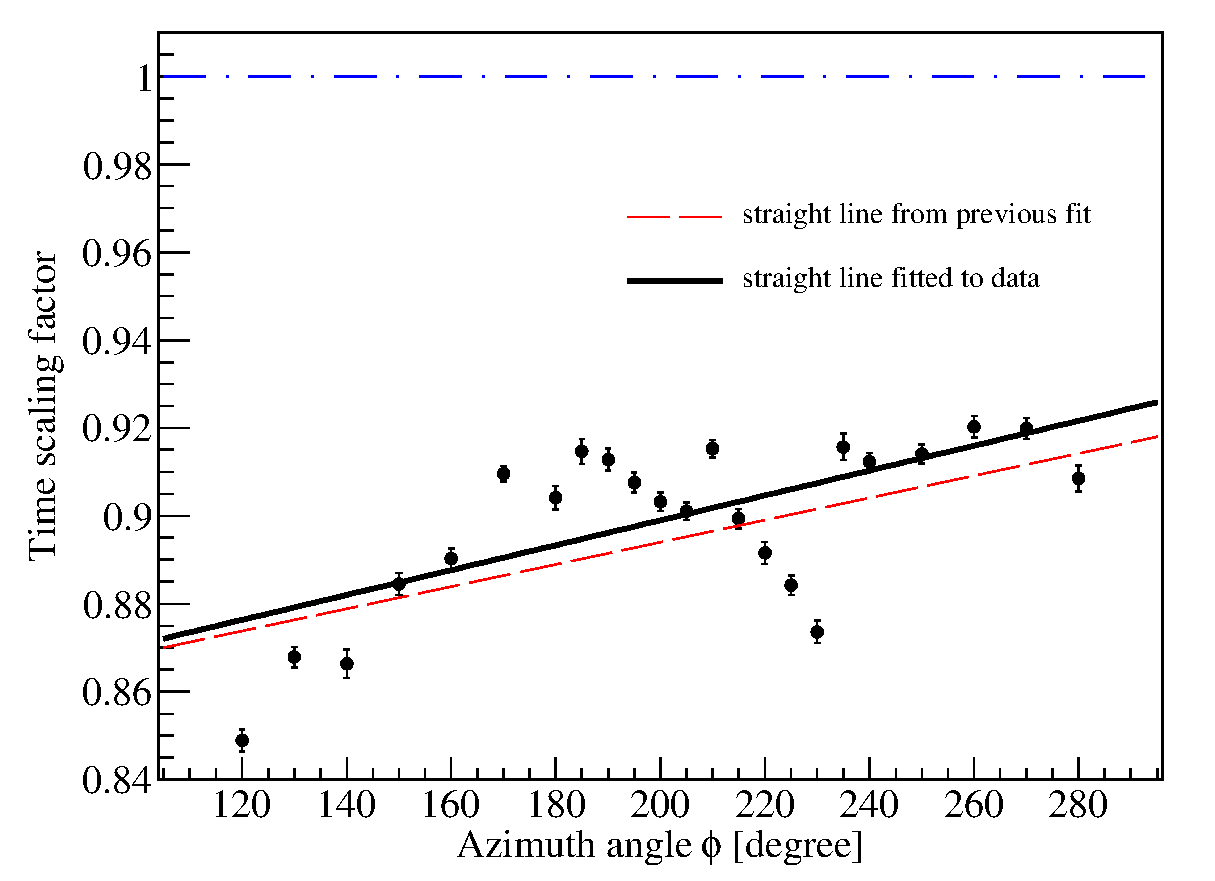
\includegraphics[width=\linewidth]{tsline}
\caption{Mean time scaling factor (black dots) for pulses simulated
for each angle individually against $\phi$. The result of a straight
line fit is given as a solid line. The shifted polynomial from
Fig.~\ref{f:tsc} is overlaid for comparison.}
\label{f:tsl}
\end{figure}

\section{Summary}
\label{s:sum}
A fully functional pulse shape simulation package has been jointly
developed by the GERDA and Majorana collaborations. Its application to
true-coaxial $n$-type germanium detectors was partially verified by
comparing to the data taken with two GERDA Phase~II prototype
detectors. The data confirm the longitudinal anisotropies inherent to
the model of the drift of charges carriers. The longitudinal
anisotropy connected to the drift of electrons was seen in the
dependence of the rise-time on the azimuthal angle, $\phi$, of the
energy deposition. After adjusting the simulation reproduces the
risetimes within $\pm$3\%.

\begin{acknowledgement}
We would like to thank people in the Monte Carlo group of the Majorana
collaboration for their kind help and cooperation in the programming.
\end{acknowledgement}

\begin{appendices}

\section{Electron drift velocity}
\label{s:elec} 
\setcounter{equation}{0}
\renewcommand{\theequation}{A.\arabic{equation}}
\setcounter{figure}{0}
\renewcommand{\thefigure}{A.\arabic{figure}}
\setcounter{footnote}{0}

In this appendix it is explained in detail how to calculate the
electron drift velocity in an arbitrary direction using the model
provided in \cite{miha} and references therein.

There are four equivalent $\langle 111 \rangle$ axes in a germanium
crystal. The equipotential surfaces of the conduction band in these
regions have ellipsoidal shapes as shown in Fig~\ref{f:valley}.

\begin{figure}[htpb]
\centering
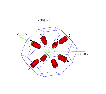
\includegraphics[width=0.6\linewidth]{valleys}   
\caption{Ellipsoidal equipotential surfaces in regions near four
equivalent $\langle 111 \rangle$ axes, where the probability density
of free electrons is dominant (taken from Ref.~\cite{bart}).}
\label{f:valley} 
\end{figure} 

The dependence of the electron drift velocity on the electric field
can be written as
\begin{equation} 
\label{e:ed} 
\vec{v}_{e}(\vec{E}) = - \mathcal{A}(E) \sum_{j} \frac{n_{j}}{n} 
\frac{\gamma_{j}\vec{E_{0}}}
{\sqrt{\vec{E_{0}}^{T}\gamma_{j}\vec{E_{0}}}}, 
j=1,2,3,4,
\end{equation} 
where the coefficient $\mathcal{A}$ is a function of $E = |\vec{E}|$;
$\vec{E_{0}}$ is the normalized electric field vector; $n_{j}/n$ is
the fraction of free electrons drifting near the $j$-th $\langle 111
\rangle$ axis and $\gamma_{j}$ is the effective mass tensor for these
electrons; the negative sign indicates that electrons drift to the
opposite direction of $\vec{E}$.

The effective mass tensor in the local coordinates $x^{\prime}
y^{\prime} z^{\prime}$ as defined in Fig.~\ref{f:axes} has a very
simple expression:
\begin{equation} 
\label{e:g0} 
\gamma_{0} \equiv \left( 
\begin{array}{ccc} 
m_{t}^{-1} & 0 & 0 \\ 
0 & m_{l}^{-1} & 0 \\ 
0 & 0 & m_{t}^{-1} 
\end{array} \right), 
\end{equation} 
where $m_{t} = 1.64m_{e}$ is the transverse effective electron mass
and $m_{l} = 0.0819m_{e}$ is the longitudinal effective electron mass,
with $m_{e}$ denoting the free electron mass. Its expressions in any
other coordinates, e.g. the $xyz$ coordinates, can be obtained by
transforming $\gamma_{0}$ from $x^{\prime} y^{\prime} z^{\prime}$ to
$xyz$ coordinates:
\begin{equation} 
\label{e:gs} 
\gamma_{j} = R_{j}^{-1}\gamma_{0}R_{j} = R_{j}^{T}\gamma_{0}R_{j}, 
\end{equation} 
where 
\begin{equation} 
\label{e:rs} 
R_{j} = R_{x^{\prime}}(\arccos(\sqrt{2/3}))R_{z}(\phi_{110}+(j-1)\pi/2) 
\end{equation} 
is the rotation matrix which aligns $x^{\prime}, y^{\prime},
z^{\prime}$ to $x,y,z$, respectively. $R_a(\alpha)$ indicates a
counter-clockwise rotation\footnote{defined as looking along the
axis.} around the axis~$a$ with rotation angle~$\alpha$.
 
\begin{figure}[htpb]
\centering
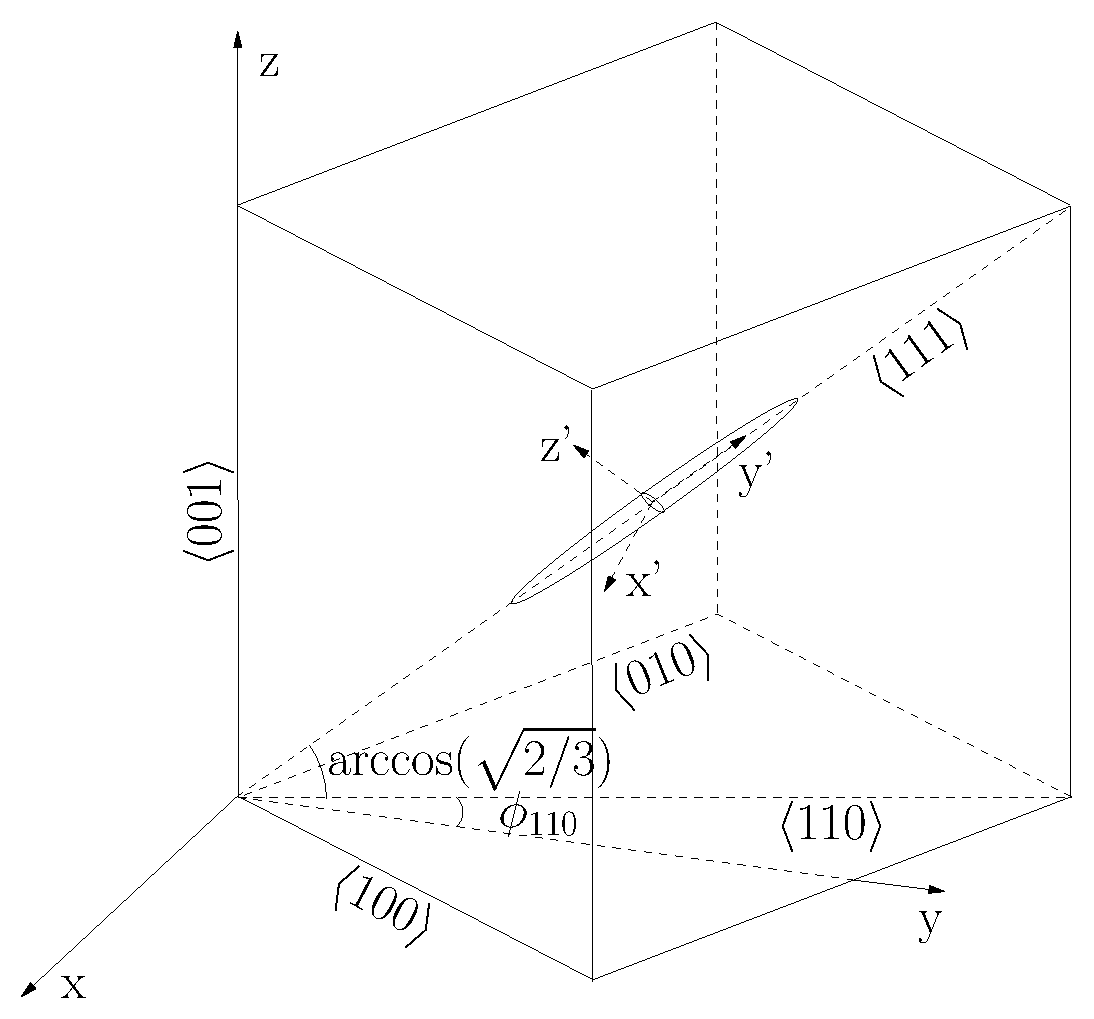
\includegraphics[width=0.7\linewidth]{axes}   
\caption{Relation between the local coordinates $x^{\prime} y^{\prime}
z^{\prime}$ and the Geant4 coordinates $xyz$. The $x^{\prime}$ axis is
perpendicular to the plane defined by $\langle111\rangle$ and $\langle
001 \rangle$.}
\label{f:axes} 
\end{figure} 

The deviation from an equal population (1/4) of free electrons is
assumed to depend on the electric field like:
\begin{equation} 
\label{e:nion} 
\frac{n_{j}}{n} = \frac{1}{4} + \mathcal{R}(E) 
\left[ \frac{\sqrt{\vec{E_{0}}^{T}\gamma_{j}\vec{E_{0}}}}
{\sum_{i}\sqrt{\vec{E_{0}}^{T}\gamma_{i}\vec{E_{0}}}} - 
\frac{1}{4} \right],  
\end{equation} 
where the coefficient $\mathcal{R}$ is a function of $E=|\vec{E}|$.
 
An electric field applied along the $\langle 100 \rangle$ direction
affects the population of the electrons in all $\langle 111 \rangle$
valleys equally, hence $n_{j}/n = 1/4$. In this case $\mathcal{A}(E)$
can be simply expressed as
\begin{equation} 
\label{e:ae} 
\mathcal{A}(E) = - \frac{v_{e}^{100}(E)}  
{\displaystyle \sum_{j} \frac{1}{4} \frac{\gamma_{j}}
{\sqrt{\vec{E}_{0}^{T}\gamma_{j}\vec{E}_{0}}}}
\end{equation}
with $\vec{E}_{0}$ parallel to $\langle 100 \rangle$, and
$v_{e}^{100}(E)$ being the drift velocity along $\langle 100 \rangle$,
which is given by Eq.~\ref{e:para}.
 
If the electric field vector is oriented along one of the four
equivalent $\langle 111 \rangle$ axes, there is a uniform population
of the electrons among the other three $\langle 111 \rangle$ axes,
namely,
\begin{equation} 
\label{e:n111} 
\frac{n_{2}}{n} = \frac{n_{3}}{n} = \frac{n_{4}}{n}. 
\end{equation} 
Since 
\begin{equation} 
\label{e:nsum} 
\displaystyle \sum_{j}\frac{n_{j}}{n} = 1, 
\end{equation} 
we have 
\begin{equation} 
\label{e:n12} 
\frac{n_{1}}{n} + 3\frac{n_{2}}{n}= 1. 
\end{equation} 
Another relation between $n_{1}/n$ and $n_{2}/n$ is obtained from
Eq.~\ref{e:ed}:
\begin{equation} 
\label{e:n12p} 
\begin{split}
- \frac{v_{e}^{111}(E)}{\mathcal{A}(E)} = &
\frac{n_{1}}{n} \frac{\gamma_{1}} 
{\sqrt{\vec{E_{0}}^{T}\gamma_{1}\vec{E_{0}}}} +
\frac{n_{2}}{n} \frac{\gamma_{2}}         
{\sqrt{\vec{E_{0}}^{T}\gamma_{2}\vec{E_{0}}}} \\ + &
\frac{n_{2}}{n} \frac{\gamma_{3}}         
{\sqrt{\vec{E_{0}}^{T}\gamma_{3}\vec{E_{0}}}} +  
\frac{n_{2}}{n} \frac{\gamma_{4}}         
{\sqrt{\vec{E_{0}}^{T}\gamma_{4}\vec{E_{0}}}}, 
\end{split}
\end{equation}
with $\vec{E_{0}}$ parallel to $\langle 111 \rangle$ and
$v_{e}^{111}(E)$ being the drift velocity along $\langle 111 \rangle$,
which is given by Eq.~\ref{e:para}. The values of $n_{1}/n$ and
$n_{2}/n$ can be obtained by solving Eqs.~\ref{e:n12} and
\ref{e:n12p}. Then $\mathcal{R}(E)$ can be calculated as
\begin{equation} 
\label{e:re} 
\mathcal{R}(E) = \frac{n_{1}/n - 1/4}
{\displaystyle \frac{\sqrt{\vec{E_{0}}^{T}\gamma_{1}\vec{E_{0}}}}
{\sum_{j}\sqrt{\vec{E_{0}}^{T}\gamma_{j}\vec{E_{0}}}} - 
\frac{1}{4}},
\end{equation} 
with $\vec{E_{0}}$ parallel to $\langle 111 \rangle$.

Once $\mathcal{A}$ and $\mathcal{R}$ are known, $\vec{v}_{e}$ can be
obtained by solving Eqs.~\ref{e:ed} and \ref{e:nion}. Since the values
of $\mathcal{A}$ and $\mathcal{R}$ are independent of $\phi_{110}$,
$\phi_{110}$ can be set to zero during the determination of
$\mathcal{A}$ and $\mathcal{R}$ so that the calculation is simplified.

\section{Hole drift velocity} 
\label{s:hole} 
\setcounter{equation}{0}
\renewcommand{\theequation}{B.\arabic{equation}}
\setcounter{figure}{0}
\renewcommand{\thefigure}{B.\arabic{figure}}

In this appendix it is explained in detail how to calculate the hole
drift velocity in an arbitrary direction using the model provided in
\cite{bart} and references therein.

It is assumed in this model that the mean wave vector
$\vec{k}_{0}(k_{0}, \theta_{0}, \phi_{0})$ of heavy holes is aligned
with the electric field $\vec{E}(E, \theta, \phi)$, namely,
$\theta_{0} = \theta, \phi_{0} = \phi$, where $\theta, \phi$ are the
polar and azimuthal angles with respect to the coordinate system
defined by the $\langle 100 \rangle$, $\langle 010 \rangle$ and
$\langle 001 \rangle$ axes. as shown in Fig.~\ref{f:vsphere}
  
\begin{figure}[htpb]
\centering
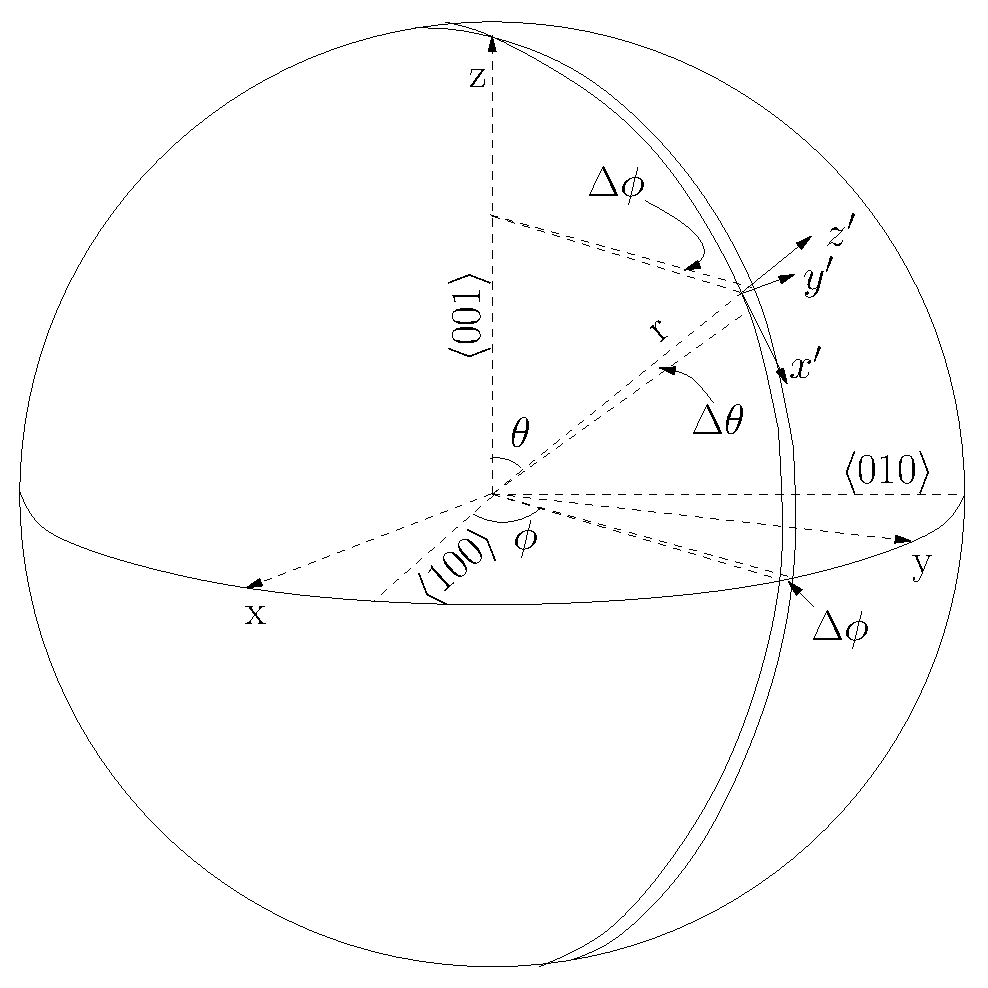
\includegraphics[width=0.8\linewidth]{vsphere}   
\caption{Relation between the crystal axes $\langle 100 \rangle$,
$\langle 010 \rangle$ and $\langle 001 \rangle$, the coordinates
$xyz$, and the local coordinates $x^{\prime} y^{\prime} z^{\prime}$.}
\label{f:vsphere} 
\end{figure} 

The three components of the hole drift velocity $\vec{v}$ in the local
coordinates, $x^{\prime} y^{\prime} z^{\prime}$, at any position $(r,
\theta, \phi)$ can be expressed as:
\begin{eqnarray*} 
\label{e:vsphere} 
v_{x^{\prime}} &=& v^{100}_{h}(E)
[1-\Lambda(k_{0})(\sin(\theta)^{4}\sin(2\phi)^{2} + \sin(2\theta)^{2})],\\ 
v_{y^{\prime}} &=& v^{100}_{h}(E)\Omega(k_{0})
[2\sin(\theta)^{3}\cos(\theta)\sin(2\phi)^{2} + \sin(4\theta)],\\ 
v_{z^{\prime}} &=& v^{100}_{h}(E)\Omega(k_{0})\sin(\theta)^{3}\sin(4\phi), 
\end{eqnarray*} 
where $v^{111}_{h}$ and $v^{100}_{h}$ are the drift velocities along
the $\langle 111 \rangle$ and $\langle 100 \rangle$ axes, which can be
calculated using Eq.~\ref{e:para}, $\Lambda$ and $\Omega$, governing
the longitudinal and transverse anisotropy of the drift, can be
expressed as
\begin{eqnarray*} 
\label{e:lamb} 
\Lambda(k_{0}) &=& -0.01322k_{0} + 0.41145k_{0}^{2} - 0.23657k_{0}^{3} + 0.04077k_{0}^{4},\\
\Omega(k_{0}) &=& 0.006550k_{0} - 0.19946k_{0}^{2} + 0.09859k_{0}^{3} - 0.01559k_{0}^{4}. 
\end{eqnarray*} 
The mean wave number $k_{0}$ can be expressed as a function of
$v_{r} = v^{111}_{h}(E)/v^{100}_{h}(E)$:
\begin{eqnarray*} 
\label{e:k0} 
k_{0}(v_{r}) = 9.2652 - 26.3467v_{r} + 29.6137v_{r}^{2} - 12.3689v_{r}^{3}. 
\end{eqnarray*} 
 
The hole drift velocity in the $xyz$ coordinates is abtained by
transforming its expression in the local coordinates $x^{\prime}
y^{\prime} z^{\prime}$ to $xyz$:
\begin{equation*} 
\label{e:v2v}   
\left( 
\begin{array}{c} 
v_{x} \\ v_{y} \\ v_{z} 
\end{array} 
\right) = R_{z}(\phi + \frac{\pi}{4} + \phi_{110}) R_{y^{\prime}}(\theta) \left(  
\begin{array}{c} 
v_{x^{\prime}} \\ v_{y^{\prime}} \\ v_{z^{\prime}} 
\end{array} \right).
\end{equation*}

\end{appendices}

\begin{thebibliography}{}
% gerda
\bibitem{Abt04}I. Abt \textit{et al.}, arXiv:hep-ex/0404039v1.
\bibitem{Sch05}S. Sch\"onert \textit{et al.}, [GERDA Collab.],
Nucl. Phys. Proc. Suppl. \textbf{145} (2005) 242.
% distinguish photon from electron
\bibitem{photon}I. Abt \textit{et al.}, Nucl. Instr. Meth. A
\textbf{583} (2007) 332.
% pulse shape analysis
\bibitem{psa}I. Abt \textit{et al.}, Eur. Phys. J. C \textbf{52}
(2007) 19.
% single compton scattering
\bibitem{scs}I. Abt \textit{et al.}, Eur. Phys. J. C \textbf{54}
(2008) 425.
% psa from Majorana
\bibitem{psam}S. R. Elliott \textit{et al.}, Nucl. Instr. Meth. A
\textbf{558} (2006) 504.
% Majorana
\bibitem{Gai03}R. Gaitskell \textit{et al.}, [Majorana Collab.]
arXiv:nucl-ex/0311013.
\bibitem{Aal04}C. E. Aalseth \textit{et al.}, [Majorana Collab.]
Phys. Atom. Nucl. \textbf{67} (2004) 2002; Yad. Fiz. \textbf{67}
(2004) 2025; arXiv:hep-ex/0405008.
% Ramo's theorem
\bibitem{Gat82}E. Gatti, \textit{et. al.},
Nucl. Instr. Meth. \textbf{193} (1982) 651.
\bibitem{Rad88}V. radeka, Ann. Rev. Nucl. Part. Sci. \textbf{38}
(1988) 217.
\bibitem{He00}Z. He, Nucl. Instr. Meth. A \textbf{463} (2000) 250.
% Geant4
\bibitem{G403}S. Agostinelli \textit{et al.}, [Geant4 Collab.],
Nucl. Instr. Meth. A \textbf{506} (2003) 250.
\bibitem{G406}J. Allison \textit{et al.}, IEEE
Trans. Nucl. Sci. \textbf{53} (2006) 207.
% MaGe paper
\bibitem{MaGe}Y. Chan \textit{et al.}, arXiv:0802.0860v1 [nucl-ex].
% mobility as a function of E
\bibitem{Kno99}G. F. Knoll, \textit{Radiation of Detection and
Measurement} third ed., (Wiley, New York 1999) 423.
% e drift
\bibitem{miha}L. Mihailescu \textit{et al.}, Nucl. Instr. Meth. A
\textbf{447} (2000) 350.
% h drift
\bibitem{reg}L. Reggiani \textit{et al.}, Phys. Rev. B \textbf{16}
(1977) 2781.
% e and h drift
\bibitem{bart}B. Bruyneel \textit{et al.}, Nucl. Instr. Meth. A
\textbf{569} (2006) 764.
\bibitem{agata}AGATA homepage, \url{http://www-w2k.gsi.de/agata/}.
\bibitem{bart2}Private conversation with B. Bruyneel, one of the
authors of Ref.~\cite{bart}.
\bibitem{heavy}E. M. Conwell, \textit{High field transport in
semiconductors, Vol. 9 of Solid State Physics}, (Academic Press,
1967).
% Siegfried I characterization
\bibitem{si}I. Abt \textit{et al.}, Nucl. Instr. Meth. A \textbf{577}
(2007) 574.

\end{thebibliography}
%
\end{document}
